% ============================================================================
% Electronic Supplementary Material (ESM)
% Induction agents for emergency tracheal intubation in critically ill adults
% ============================================================================
\documentclass[11pt]{article}

\usepackage[utf8]{inputenc}
\usepackage[T1]{fontenc}
\usepackage{lmodern}
\usepackage[margin=1in]{geometry}
\usepackage{graphicx}
\usepackage{booktabs}
\usepackage{array}
\usepackage{tabularx}
\usepackage{multirow}
\usepackage{longtable}
\usepackage[hidelinks]{hyperref}
\usepackage{setspace}
\usepackage{caption}
\usepackage{float}
\usepackage{pdfpages}
\usepackage{pdflscape}

\onehalfspacing

\newcolumntype{L}[1]{>{\raggedright\arraybackslash}p{#1}}
\newcolumntype{C}[1]{>{\centering\arraybackslash}p{#1}}

% Counters for eFigures/eTables
\newcounter{efigure}
\renewcommand{\theefigure}{e\arabic{efigure}}
\newcounter{etable}
\renewcommand{\theetable}{e\arabic{etable}}
\newenvironment{efigure}[1][htbp]{\refstepcounter{efigure}\begin{figure}[#1]}{\end{figure}}
\newenvironment{etabletab}[1][htbp]{\refstepcounter{etable}\begin{table}[#1]}{\end{table}}

\begin{document}

\begin{center}
{\LARGE\bfseries Electronic Supplementary Material}\\[12pt]
{\large Induction agents for emergency tracheal intubation in critically ill adults: a systematic review and network meta-analysis}\\[8pt]
{\normalsize Zampieri FG, Schmidt RC, Besen BAMP, Ramos FJDS, Lamontagne F, Adhikari NKJ, Freitas FGR, Machado FR}\\[4pt]
{\normalsize for the PROMINE Investigators}
\end{center}

\vspace{1cm}
\tableofcontents
\newpage

% ============================================================================
% APPENDIX A: SEARCH STRATEGIES
% ============================================================================
\section{Search Strategies}
\label{sec:search}

Searches were conducted from database inception through December 2025. No language restrictions were applied in the search; however, only English-language publications were included at the screening stage, with one exception: a Turkish-language study (Cinar 2011) was retained because sufficient information was available from its English abstract and AI-assisted translation.

\subsection{MEDLINE (via PubMed)}

Search executed on December 10, 2025.

\begin{verbatim}
(
  "Intubation, Intratracheal"[Mesh] OR intubat*[tiab] OR
  "tracheal intubation"[tiab] OR "rapid sequence"[tiab] OR
  "rapid-sequence"[tiab] OR RSI[tiab]
)
AND
(
  "Emergency Service, Hospital"[Mesh] OR
  "Intensive Care Units"[Mesh] OR
  emergency[tiab] OR "emergency department"[tiab] OR ED[tiab] OR
  "critical illness"[Mesh] OR "critically ill"[tiab] OR
  ICU[tiab] OR "prehospital"[tiab]
)
AND
(
  etomidate[tiab] OR ketamine[tiab] OR propofol[tiab] OR
  amidate[tiab] OR diprivan[tiab] OR ketofol[tiab]
)
AND
(
  randomized controlled trial[pt] OR controlled clinical trial[pt] OR
  random*[tiab] OR trial[tiab] OR "clinical trial"[pt]
)
NOT
(
  animals[mh] NOT humans[mh]
)
\end{verbatim}

\subsection{Embase (via Ovid)}

Search executed on December 10, 2025.

\begin{verbatim}
1.  exp endotracheal intubation/ or exp rapid sequence induction/
2.  (intubat* or "tracheal intubation" or "rapid sequence"
    or "rapid-sequence" or RSI).ti,ab.
3.  1 or 2
4.  exp emergency ward/ or exp intensive care unit/
    or exp critical illness/
5.  (emergency or "emergency department" or ED
    or "critically ill" or ICU or prehospital).ti,ab.
6.  4 or 5
7.  (etomidate or ketamine or propofol or amidate
    or diprivan or ketofol).ti,ab.
8.  exp etomidate/ or exp ketamine/ or exp propofol/
9.  7 or 8
10. 3 and 6 and 9
11. randomized controlled trial/ or controlled clinical trial/
12. (random* or trial or RCT).ti,ab.
13. 11 or 12
14. 10 and 13
15. (animal/ or nonhuman/) not human/
16. 14 not 15
\end{verbatim}

\subsection{Forward citation searching}

Forward citation searching was performed on all included trials using Google Scholar. Reference lists of recent systematic reviews (Kotani 2023, Koroki 2024, Daghmouri 2025, de Morais 2025) were also screened. No additional eligible studies were identified beyond those captured by the database searches.

\subsection{Trial registry screening}

ClinicalTrials.gov and WHO ICTRP were screened for completed or ongoing trials comparing eligible induction agents for emergency intubation. One registered trial (NCT05092152, PROMINE) was identified and included based on manuscript data. No additional eligible completed trials were identified.

\newpage

% ============================================================================
% APPENDIX B: PRISMA-NMA CHECKLIST
% ============================================================================
\section{PRISMA Extension for Network Meta-Analysis Checklist}
\label{sec:prisma-nma}

The following checklist is based on the PRISMA extension statement for systematic reviews incorporating network meta-analyses (Hutton et al., \textit{Ann Intern Med} 2015;162:777--784). Items marked with ``S'' are NMA-specific additions.

\begin{small}
\begin{longtable}{L{2.5cm} C{0.5cm} L{7.5cm} L{3.5cm}}
\toprule
\textbf{Section/Topic} & \textbf{\#} & \textbf{Checklist Item} & \textbf{Reported In} \\
\midrule
\endfirsthead
\toprule
\textbf{Section/Topic} & \textbf{\#} & \textbf{Checklist Item} & \textbf{Reported In} \\
\midrule
\endhead
\midrule
\multicolumn{4}{r}{\footnotesize\itshape Continued on next page} \\
\endfoot
\bottomrule
\endlastfoot
\multicolumn{4}{l}{\textit{\textbf{Title}}} \\
Title & 1 & Identify the report as a systematic review incorporating a network meta-analysis & Title \\[4pt]
\multicolumn{4}{l}{\textit{\textbf{Abstract}}} \\
Structured summary & 2 & Provide a structured summary & Abstract \\[4pt]
\multicolumn{4}{l}{\textit{\textbf{Introduction}}} \\
Rationale & 3 & Describe the rationale for the review, including why a network meta-analysis was conducted & Introduction, para 3 \\
Objectives & 4 & Explicit statement of questions with reference to PICOS & Introduction, para 4 \\[4pt]
\multicolumn{4}{l}{\textit{\textbf{Methods}}} \\
Protocol \& registration & 5 & Indicate existence of protocol and registration & Methods, para 1 \\
Eligibility criteria & 6 & Specify study characteristics and eligible treatments in the network & Eligibility criteria \\
Information sources & 7 & Describe all information sources & Information sources \\
Search & 8 & Full electronic search strategy for at least one database & ESM, Search Strategies \\
Study selection & 9 & State the process for selecting studies & Study selection \\
Data collection & 10 & Describe data extraction methods and confirmation processes & Study selection \\
Data items & 11 & List and define all variables sought & Outcomes; ESM data extractions \\
Geometry of the network & S1 & Describe methods to explore network geometry and potential biases & Statistical analysis; Figure 3A \\
Risk of bias in studies & 12 & Describe methods for assessing risk of bias & Risk of bias assessment \\
Summary measures & 13 & State principal summary measures; describe treatment rankings & Statistical analysis \\
Planned methods of analysis & 14 & Methods of combining results, handling multi-arm trials, variance structure & Statistical analysis \\
Inconsistency & S2 & Statistical methods to evaluate consistency of direct and indirect evidence & Statistical analysis \\
Risk of bias across studies & 15 & Assessment of cumulative evidence bias & Certainty of evidence \\
Additional analyses & 16 & Methods of additional analyses, indicating pre-specified & Subgroup and sensitivity \\[4pt]
\multicolumn{4}{l}{\textit{\textbf{Results}}} \\
Study selection & 17 & Numbers screened, assessed, included, with flow diagram & Study selection; Figure 1 \\
Network structure & S3 & Network graph for visualization & Figure 3A \\
Network geometry summary & S4 & Overview of network characteristics, gaps, potential biases & Study characteristics; Discussion \\
Study characteristics & 18 & Characteristics and citations for each study & Table 1; ESM extractions \\
Risk of bias in studies & 19 & Risk of bias for each study & Figure 2; ESM eFigures \\
Individual study results & 20 & Summary data for each treatment group, effect estimates & ESM data extractions \\
Synthesis of results & 21 & Results of each meta-analysis with confidence intervals; league tables or rankings & Results; Table 2; eFigures \\
Inconsistency & S5 & Results from investigations of inconsistency & Primary outcome \\
Risk of bias across studies & 22 & Results of bias assessment across studies & Certainty of evidence; ESM \\
Additional analyses & 23 & Results of sensitivity or subgroup analyses & Subgroup and sensitivity; ESM eFigures \\[4pt]
\multicolumn{4}{l}{\textit{\textbf{Discussion}}} \\
Summary of evidence & 24 & Main findings including strength of evidence & Discussion, paras 1--3 \\
Limitations & 25 & Limitations at study, outcome, and review level & Discussion, para 5 \\
Conclusions & 26 & General interpretation and implications for future research & Conclusions \\[4pt]
\multicolumn{4}{l}{\textit{\textbf{Funding}}} \\
Funding & 27 & Sources of funding and role of funders & Title page \\
\end{longtable}
\end{small}

\newpage

% ============================================================================
% APPENDIX C: SUPPLEMENTARY FIGURES
% ============================================================================
\section{Supplementary Figures}
\label{sec:efigures}

% --- eFigure 1: NMA forest (all treatments vs Etomidate) ---
\begin{efigure}[p]
\centering
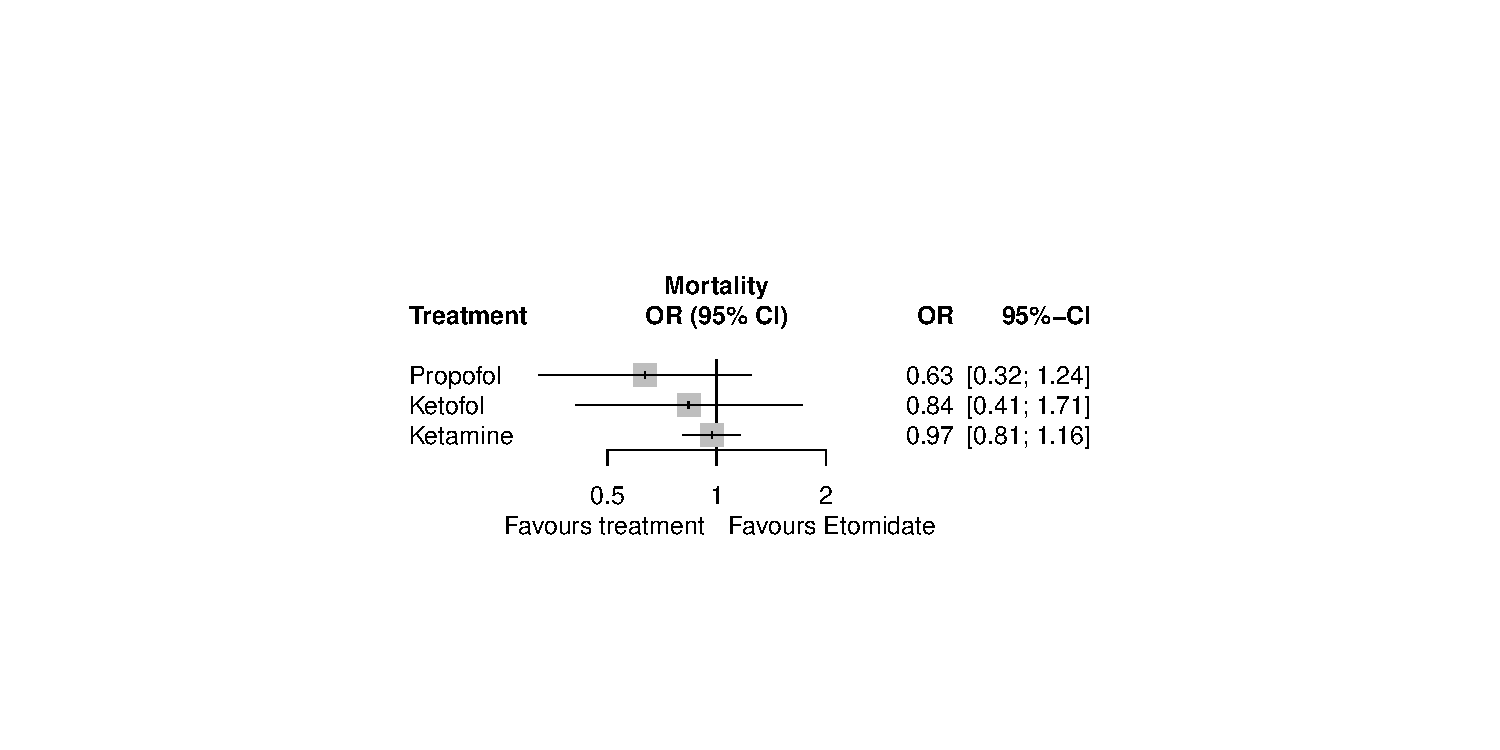
\includegraphics[width=0.85\textwidth]{eFigure1_NMA_forest_mortality.pdf}
\caption*{\textbf{eFigure~\theefigure.} Network meta-analysis forest plot for short-term mortality. All treatments compared with etomidate (reference). Random-effects model. OR $<$ 1 favors the comparator treatment (lower mortality).}
\end{efigure}

% --- eFigure 2: CV collapse ---
\begin{efigure}[p]
\centering
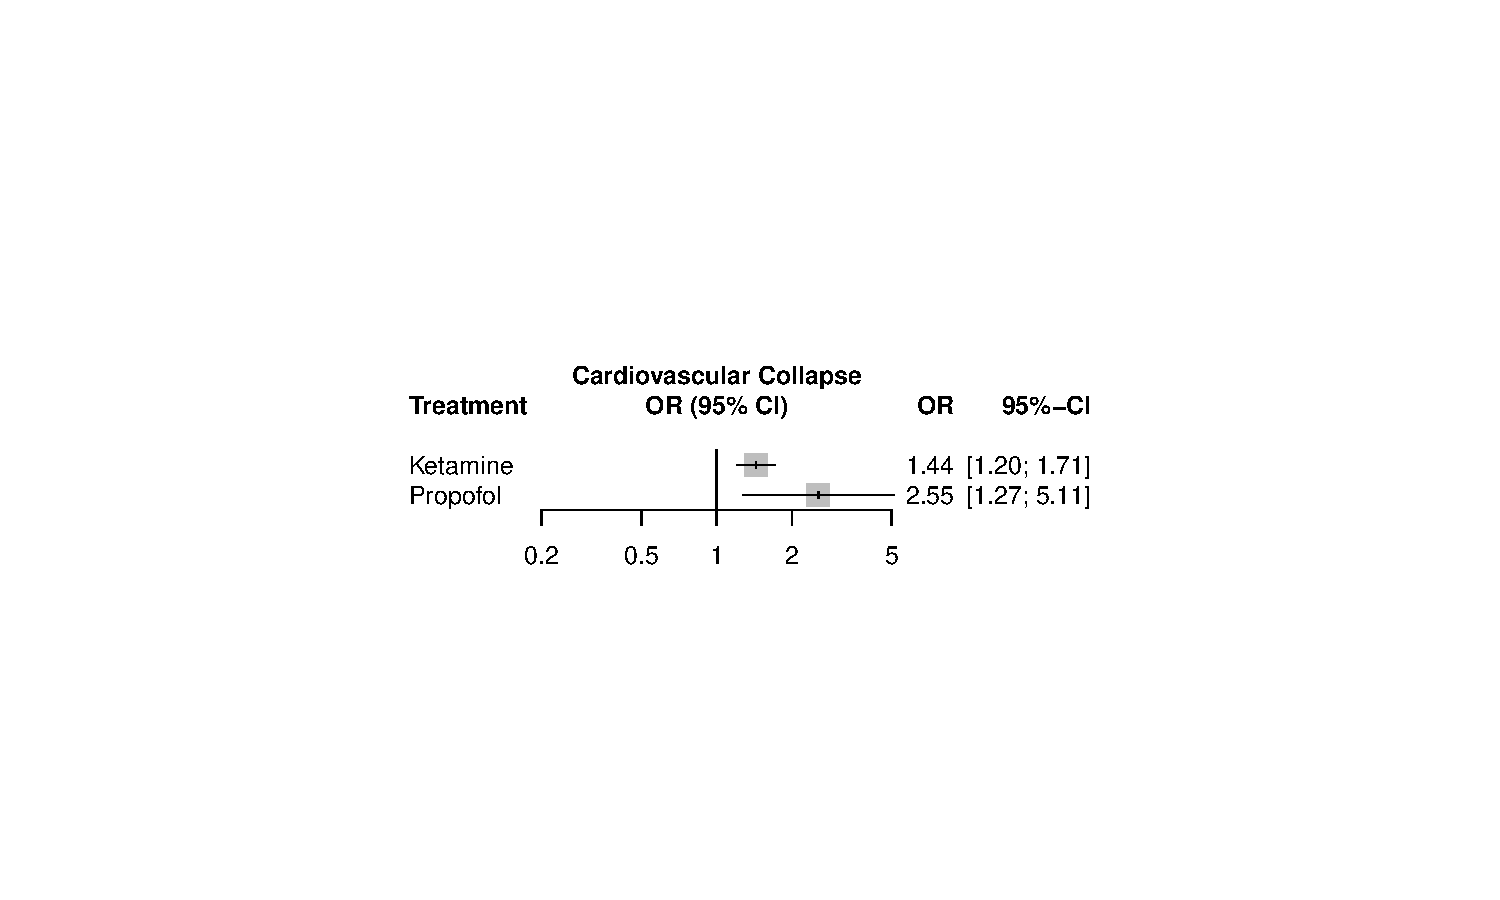
\includegraphics[width=0.85\textwidth]{eFigure2_forest_cv_collapse.pdf}
\caption*{\textbf{eFigure~\theefigure.} Forest plot for cardiovascular collapse. Three studies contributed to a three-node NMA (etomidate, ketamine, propofol). OR $>$ 1 indicates higher event rate vs etomidate.}
\end{efigure}

% --- eFigure 3: Hypotension ---
\begin{efigure}[p]
\centering
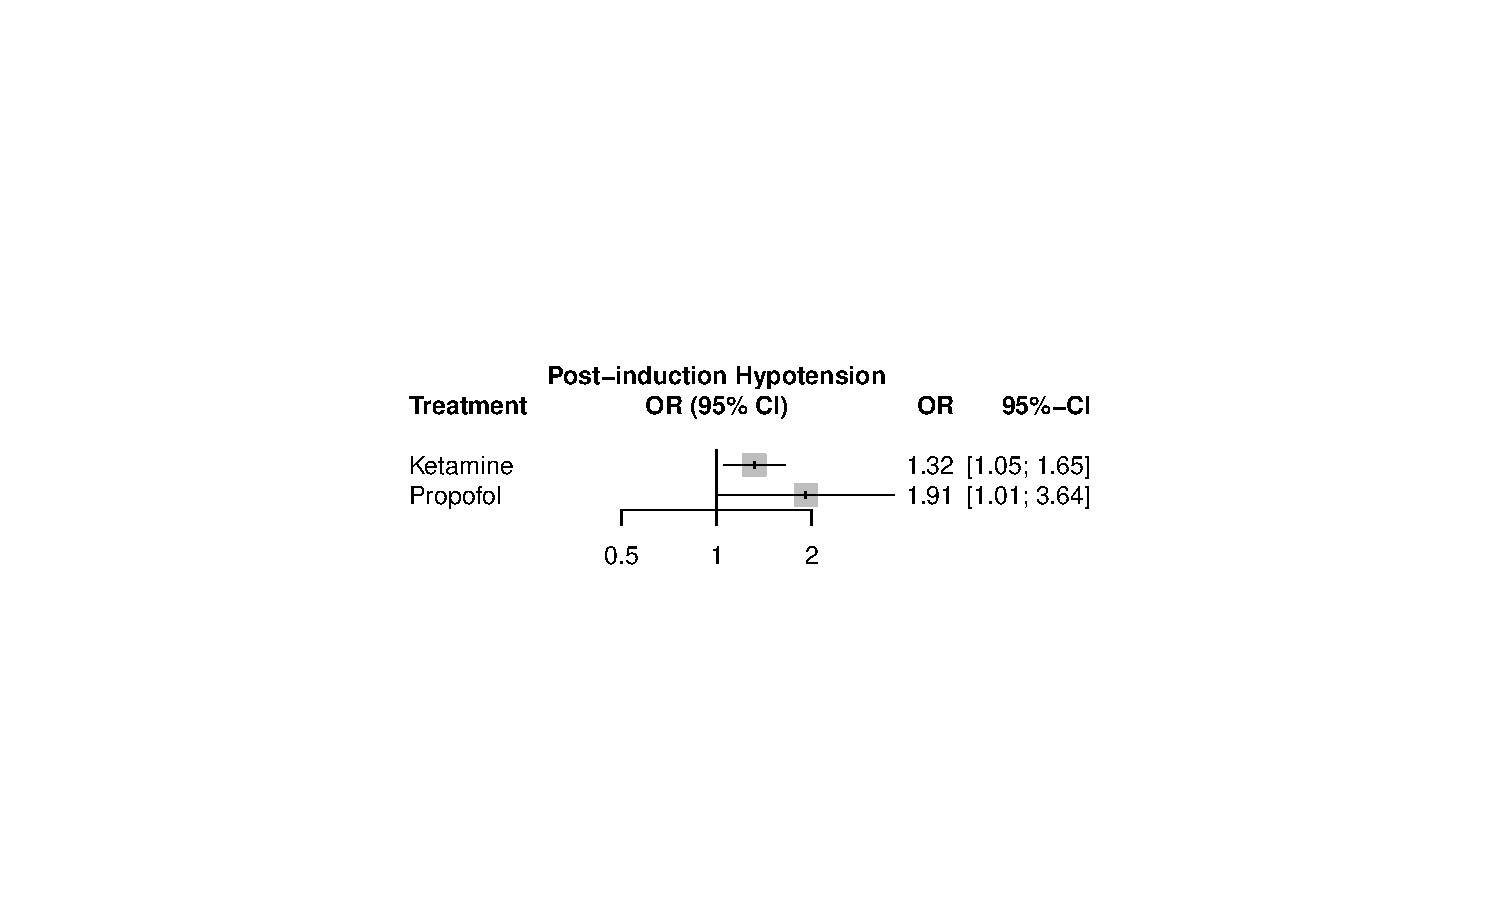
\includegraphics[width=0.85\textwidth]{eFigure3_forest_hypotension.pdf}
\caption*{\textbf{eFigure~\theefigure.} Forest plot for post-induction hypotension. Four studies contributed; definitions varied across studies (SBP $<$80, SBP $<$90, or MAP $<$65 mmHg).}
\end{efigure}

% --- eFigure 4: First-pass success ---
\begin{efigure}[p]
\centering
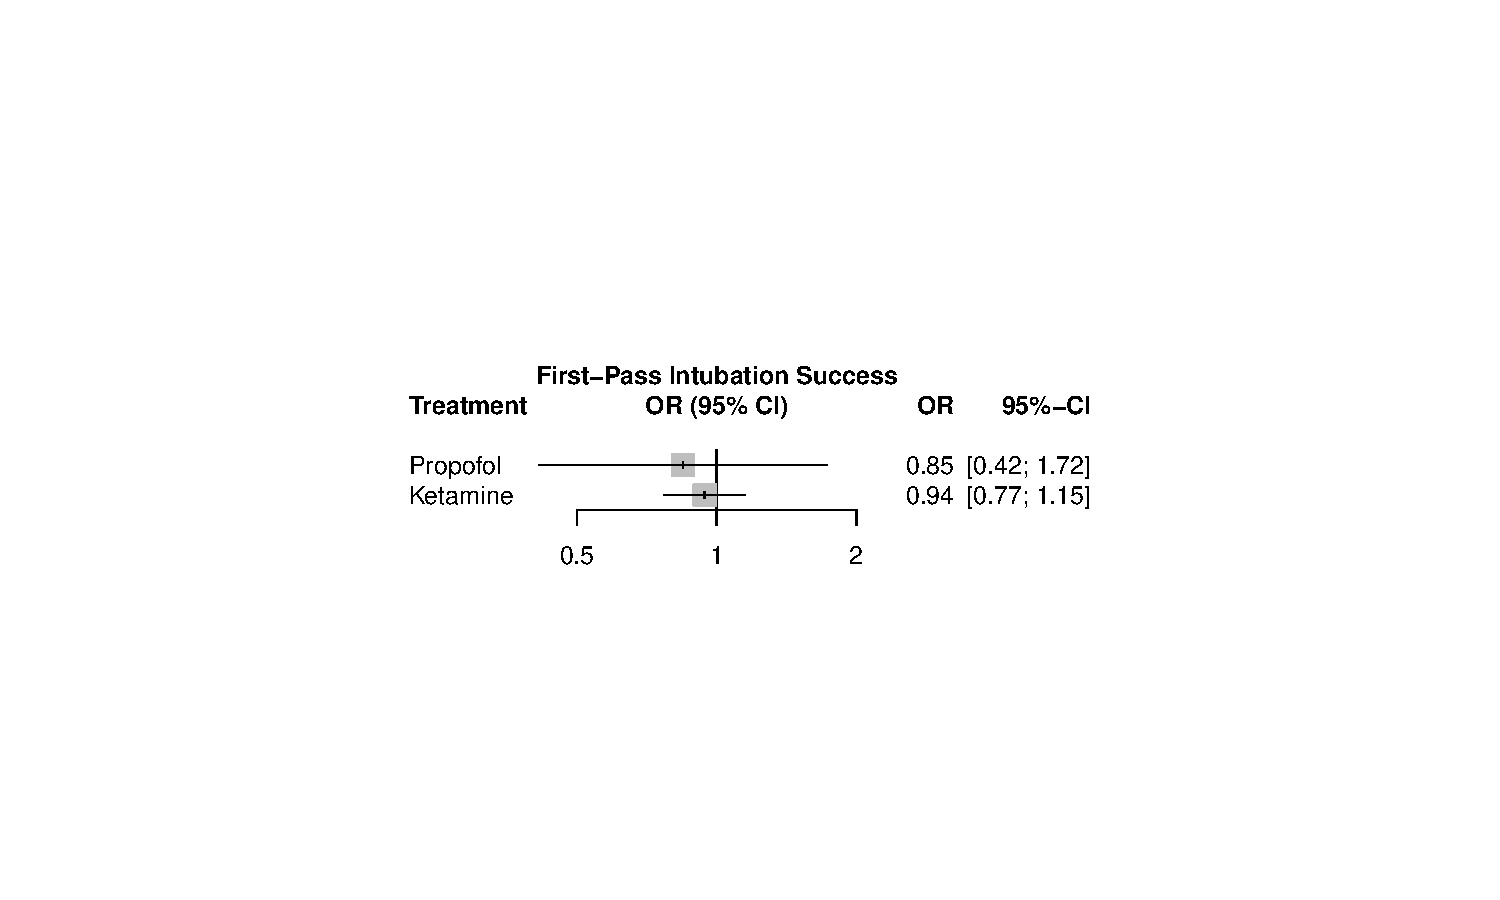
\includegraphics[width=0.85\textwidth]{eFigure4_forest_first_pass.pdf}
\caption*{\textbf{eFigure~\theefigure.} Forest plot for first-pass intubation success. Five studies contributed. OR $<$ 1 indicates lower first-pass success vs etomidate.}
\end{efigure}

% --- eFigure 5: Cardiac arrest ---
\begin{efigure}[p]
\centering
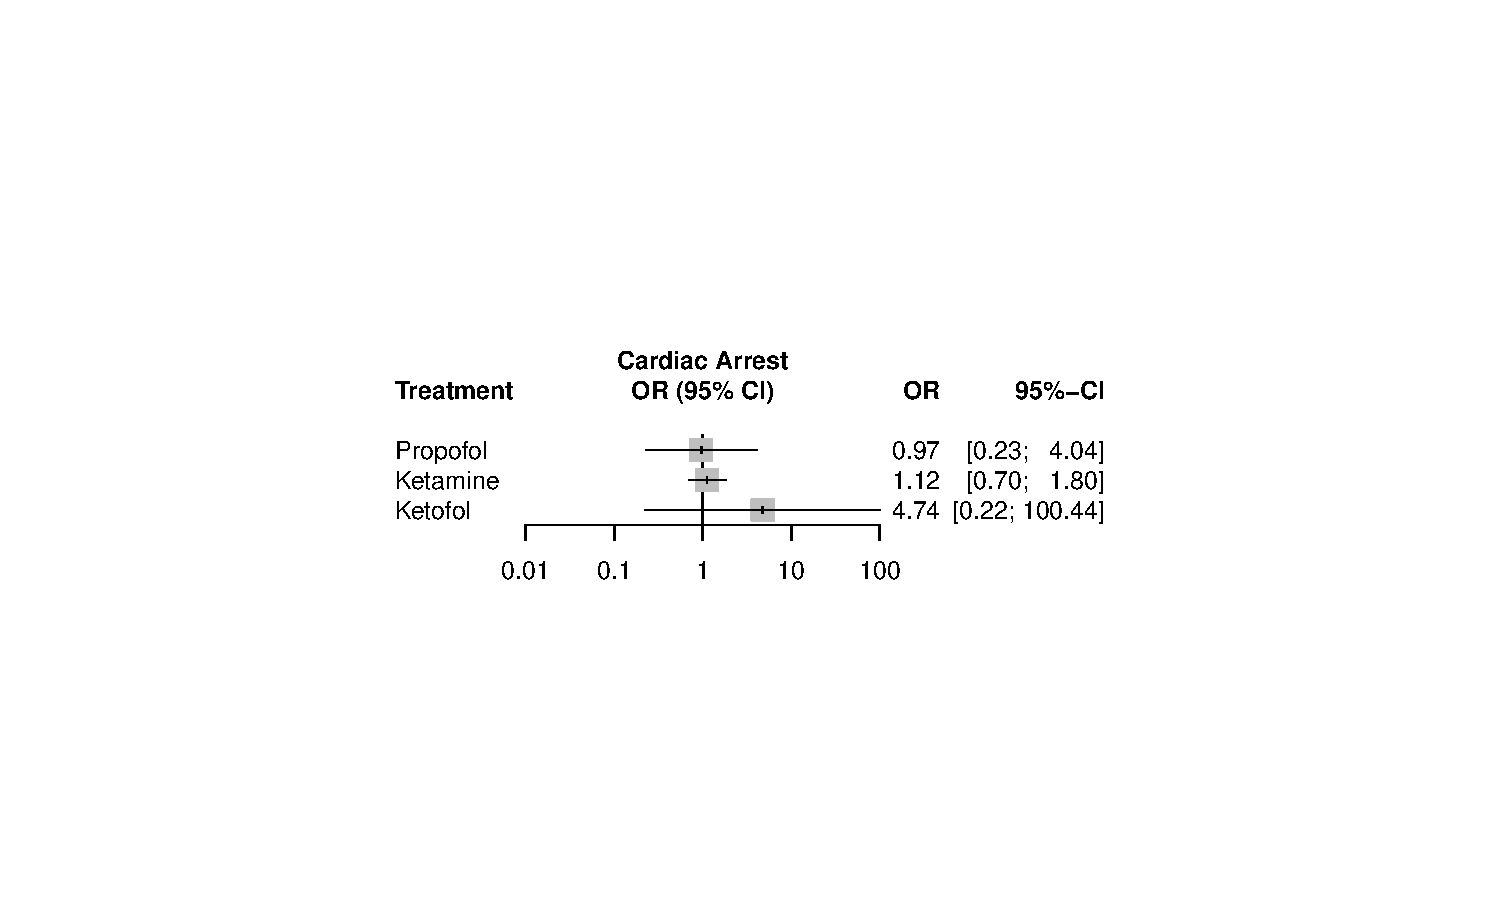
\includegraphics[width=0.85\textwidth]{eFigure5_forest_cardiac_arrest.pdf}
\caption*{\textbf{eFigure~\theefigure.} Forest plot for peri-intubation cardiac arrest. Seven studies contributed. Event rates were low across all studies.}
\end{efigure}

% --- eFigure 6: Vasopressor peri-intubation ---
\begin{efigure}[p]
\centering
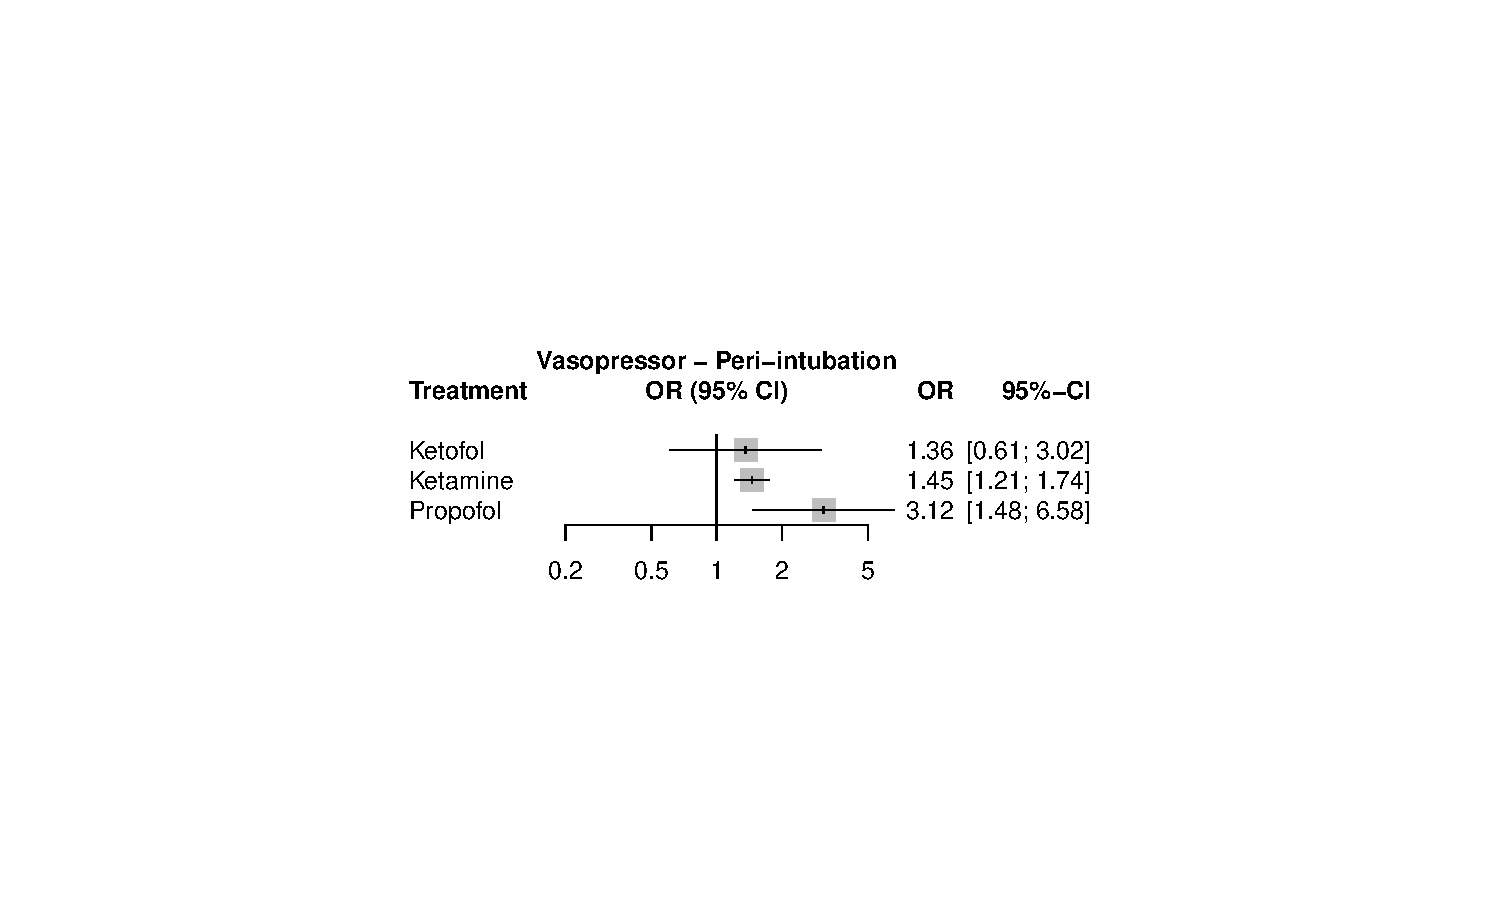
\includegraphics[width=0.85\textwidth]{eFigure6_forest_vaso_peri.pdf}
\caption*{\textbf{eFigure~\theefigure.} Forest plot for vasopressor use, peri-intubation (induction to 2--5 minutes). Five studies contributed.}
\end{efigure}

% --- eFigure 7: Vasopressor 24h ---
\begin{efigure}[p]
\centering
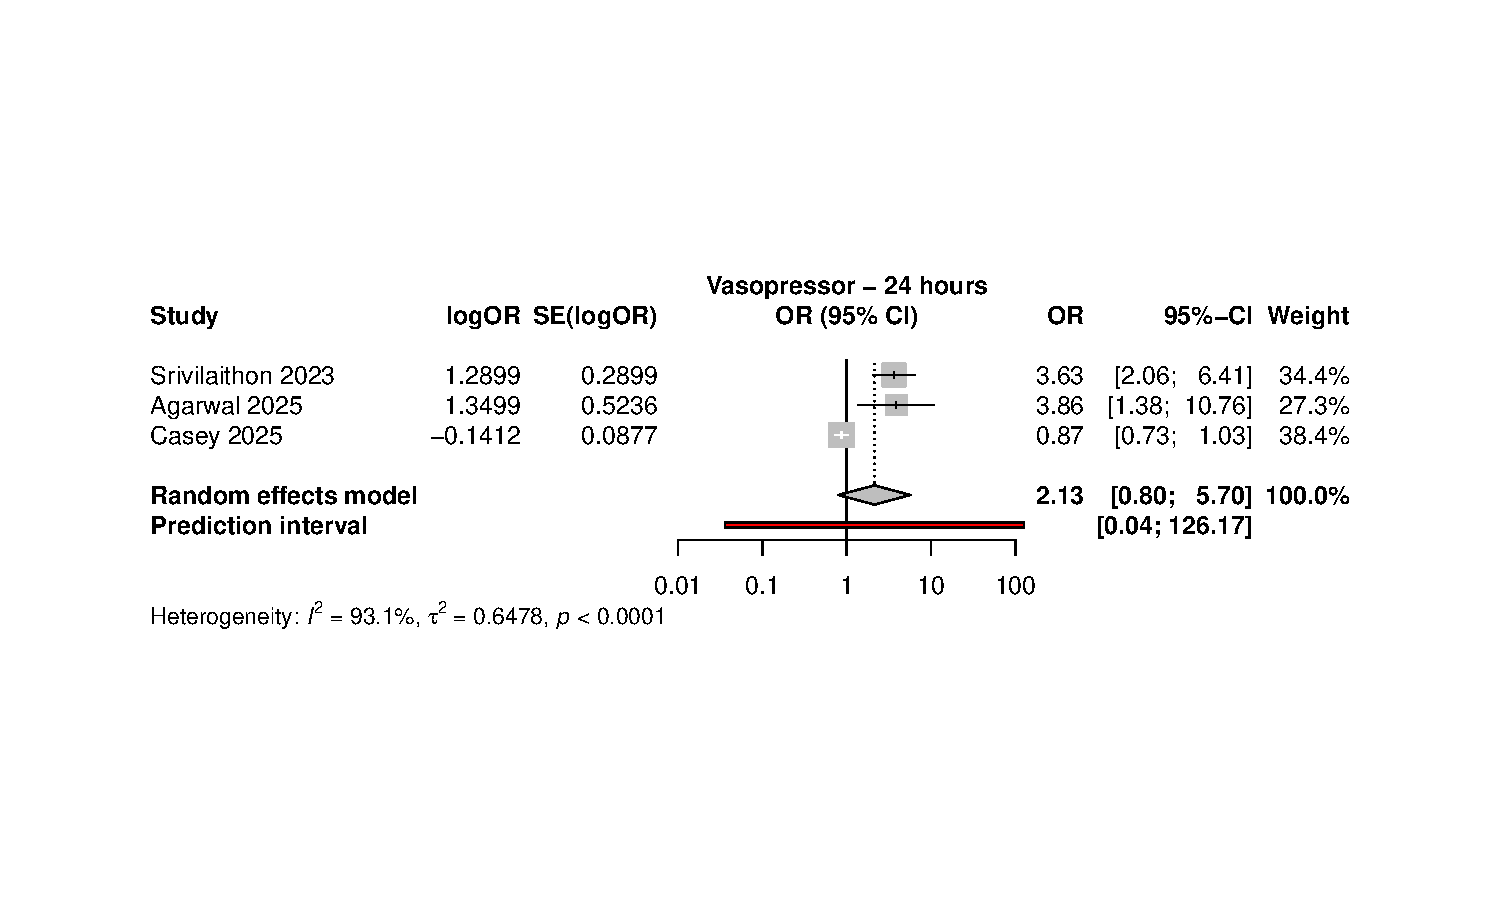
\includegraphics[width=0.85\textwidth]{eFigure7_forest_vaso_24h.pdf}
\caption*{\textbf{eFigure~\theefigure.} Forest plot for vasopressor use at 24 hours (etomidate vs ketamine direction; OR $>$ 1 indicates higher rate with etomidate). Two studies contributed. Substantial heterogeneity ($I^2$ = 96\%) precludes reliable pooled estimation. Individual study ORs were 1.15 (Casey 2025) and 3.63 (Srivilaithon 2023). In Table~2, this result is presented in the ketamine vs etomidate direction (OR 0.58, 95\% CI 0.14--2.33).}
\end{efigure}

% --- eFigure 8: Funnel plot ---
\begin{efigure}[p]
\centering
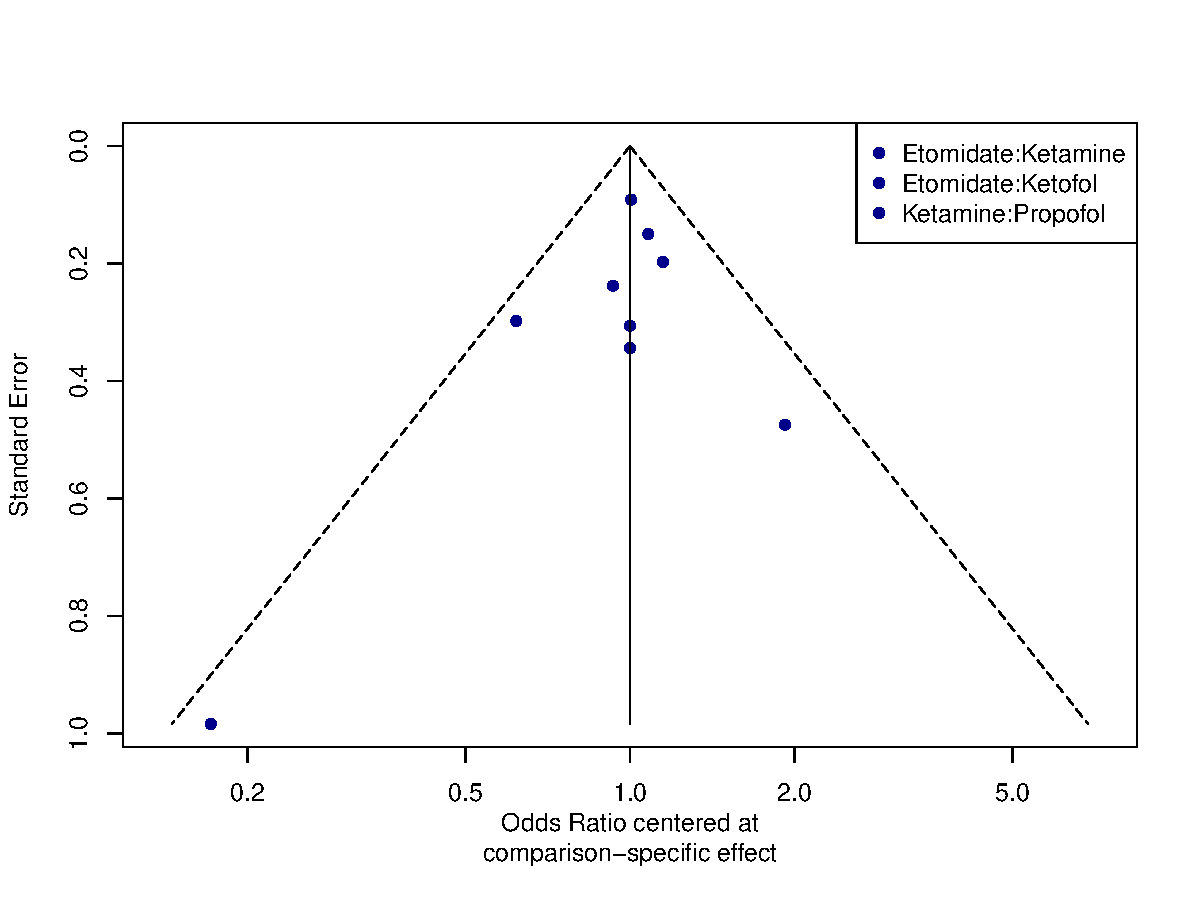
\includegraphics[width=0.75\textwidth]{eFigure8_funnel_mortality.pdf}
\caption*{\textbf{eFigure~\theefigure.} Comparison-adjusted funnel plot for the mortality network meta-analysis. No clear asymmetry was observed, although interpretation is limited by the small number of studies.}
\end{efigure}

% --- eFigure 9: Subgroup by setting ---
\begin{efigure}[p]
\centering
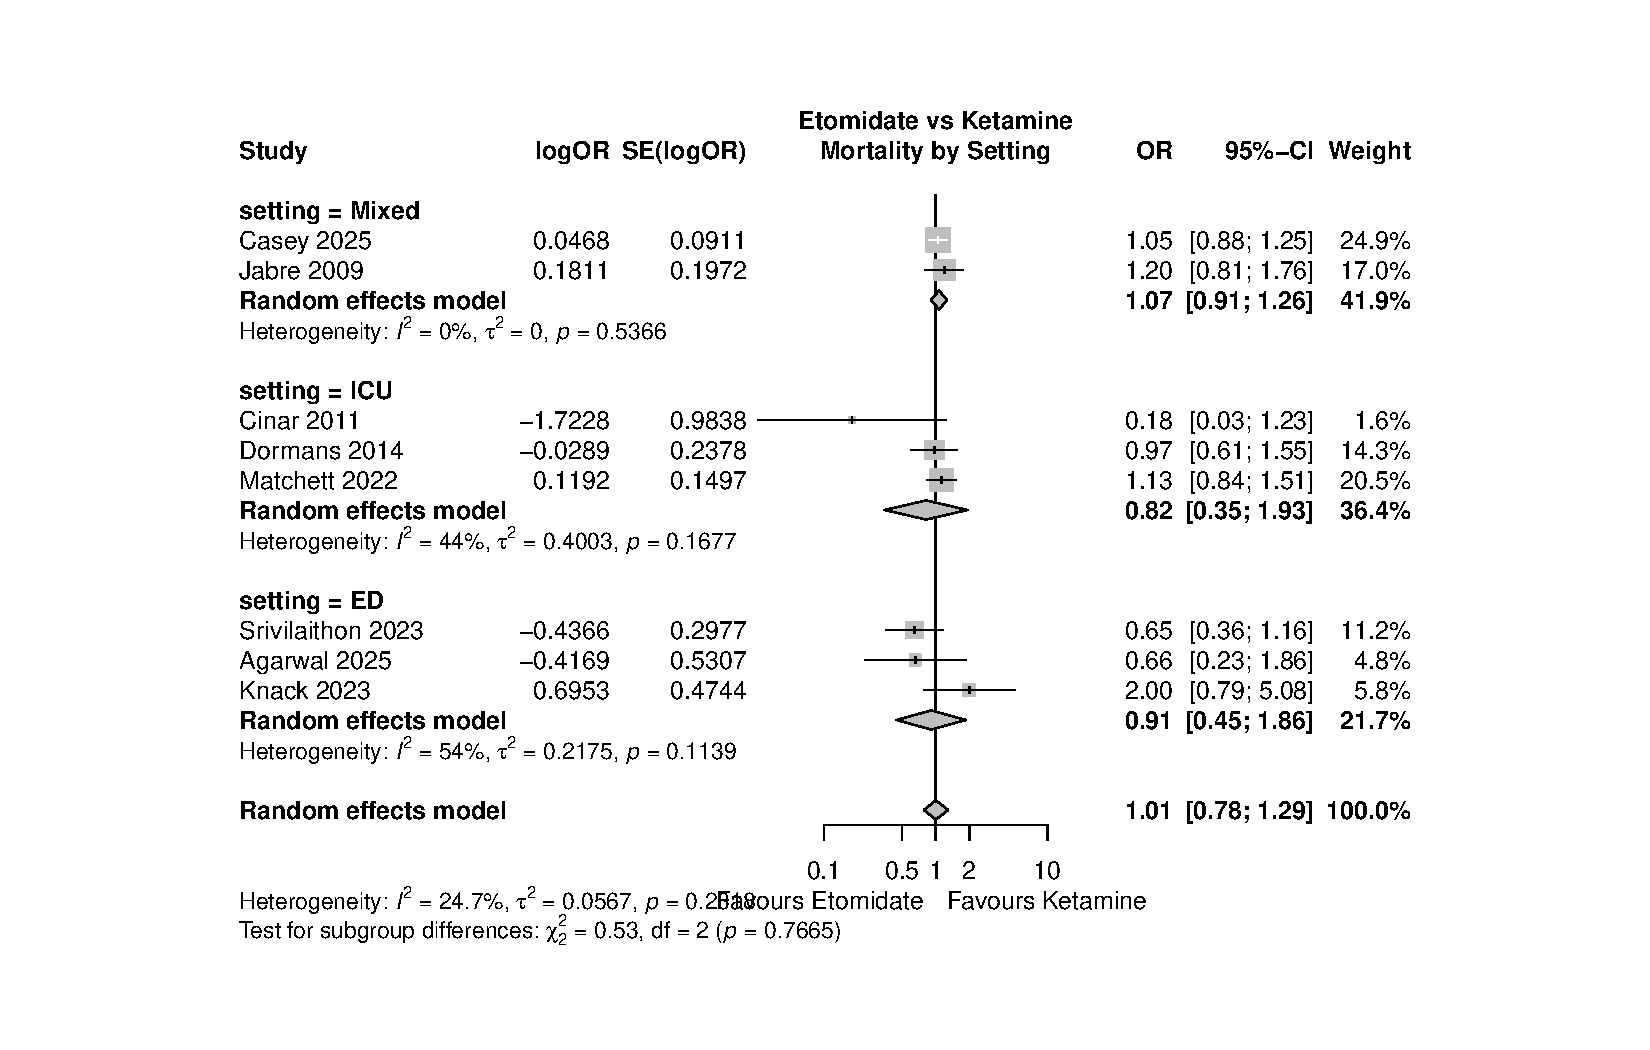
\includegraphics[width=0.9\textwidth]{eFigure9_subgroup_setting.pdf}
\caption*{\textbf{eFigure~\theefigure.} Subgroup analysis for etomidate vs ketamine mortality by clinical setting (ED, ICU, mixed). Test for subgroup differences: $p$ = 0.83. No evidence of effect modification by setting.}
\end{efigure}

% --- eFigure 10: Subgroup by RoB ---
\begin{efigure}[p]
\centering
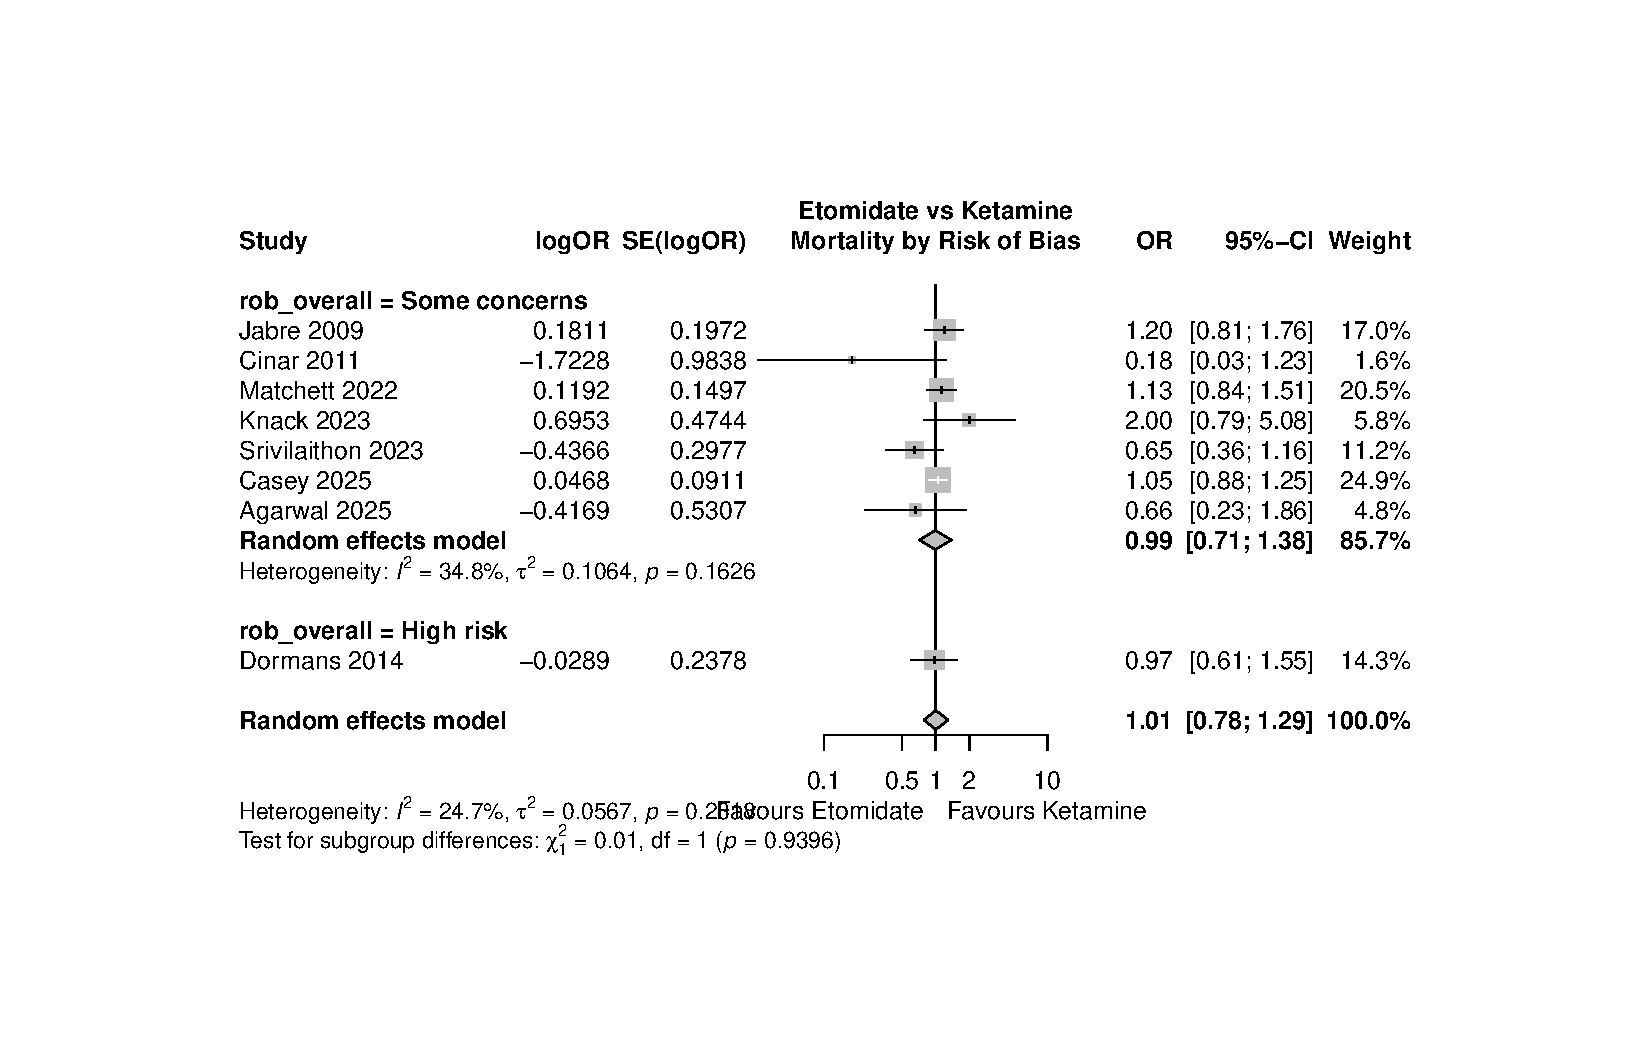
\includegraphics[width=0.9\textwidth]{eFigure10_subgroup_rob.pdf}
\caption*{\textbf{eFigure~\theefigure.} Subgroup analysis for etomidate vs ketamine mortality by overall risk of bias. Test for subgroup differences: $p$ = 0.88. Only one study (Punt 2014) was rated ``high risk.''}
\end{efigure}

% --- eFigure 11: ICU subgroup NMA ---
\begin{efigure}[p]
\centering
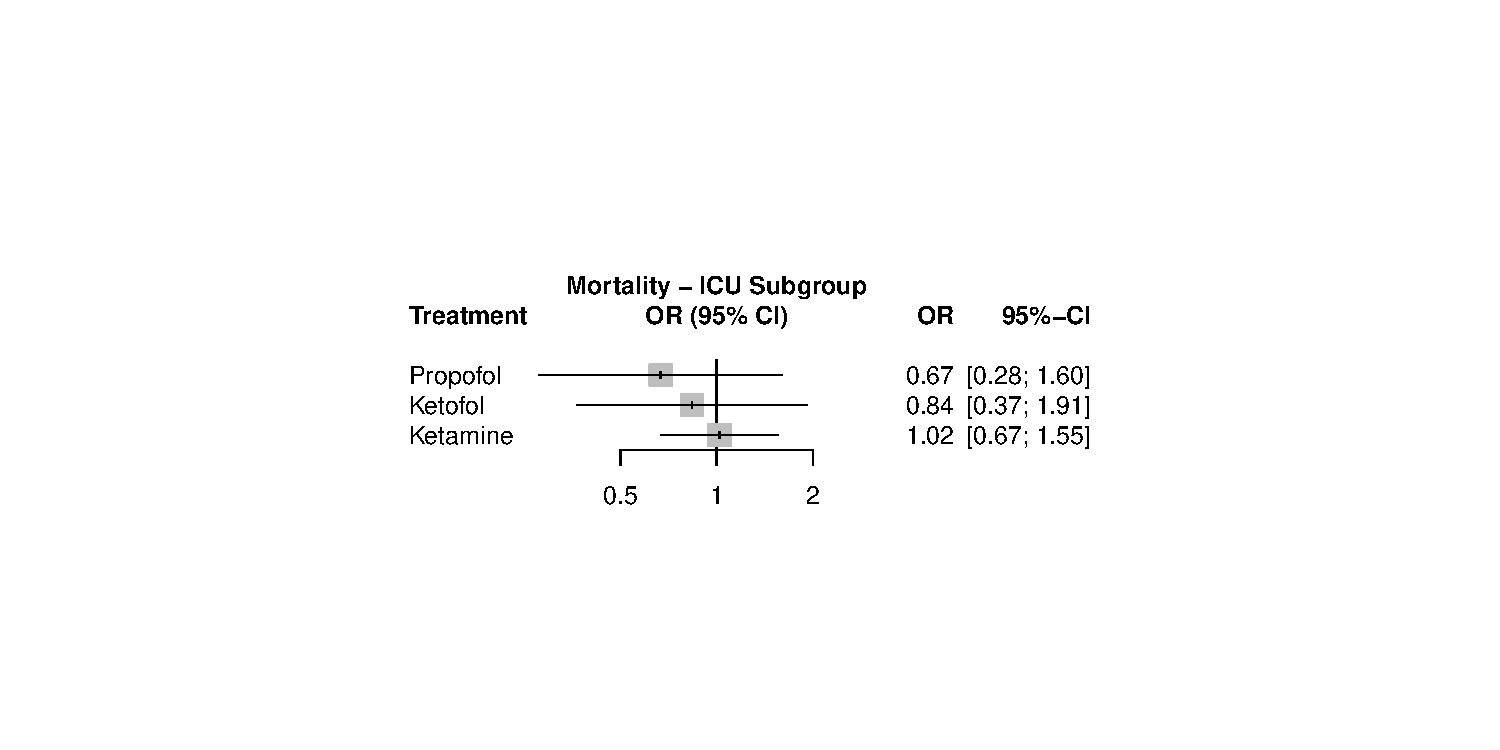
\includegraphics[width=0.85\textwidth]{eFigure11_subgroup_ICU_nma.pdf}
\caption*{\textbf{eFigure~\theefigure.} Network meta-analysis restricted to ICU studies (5 studies: Cinar, Punt, Smischney, Matchett, Schmidt). This subgroup includes all four treatment nodes with a connected network.}
\end{efigure}

% --- eFigure 12--16: Sensitivity analyses ---
\begin{efigure}[p]
\centering
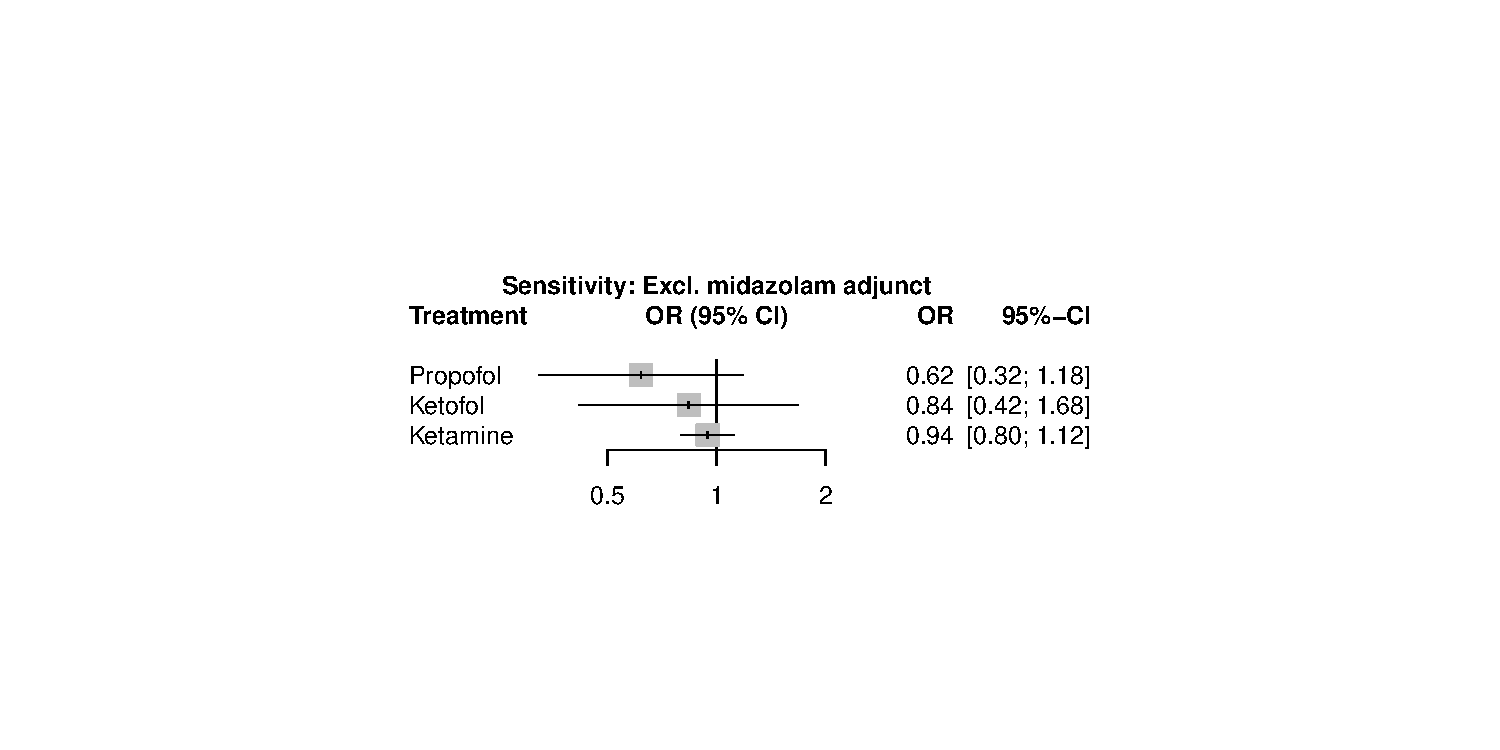
\includegraphics[width=0.85\textwidth]{eFigure12_sens_no_midaz.pdf}
\caption*{\textbf{eFigure~\theefigure.} Sensitivity analysis excluding studies with midazolam adjunct in the ketamine arm (Cinar 2011, Punt 2014 excluded; 7 studies remaining).}
\end{efigure}

\begin{efigure}[p]
\centering
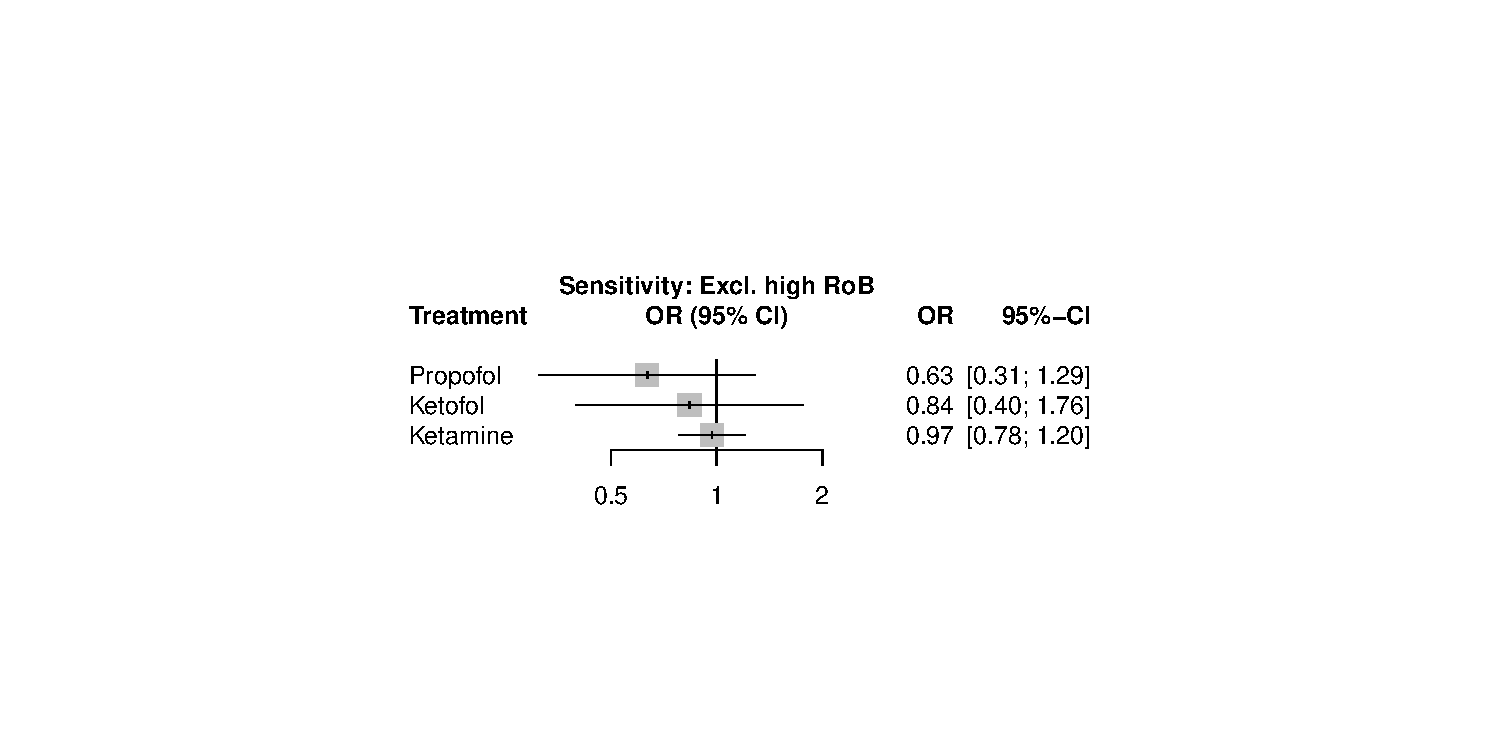
\includegraphics[width=0.85\textwidth]{eFigure13_sens_no_high_rob.pdf}
\caption*{\textbf{eFigure~\theefigure.} Sensitivity analysis excluding high risk-of-bias studies (Punt 2014 excluded; 8 studies remaining).}
\end{efigure}

\begin{efigure}[p]
\centering
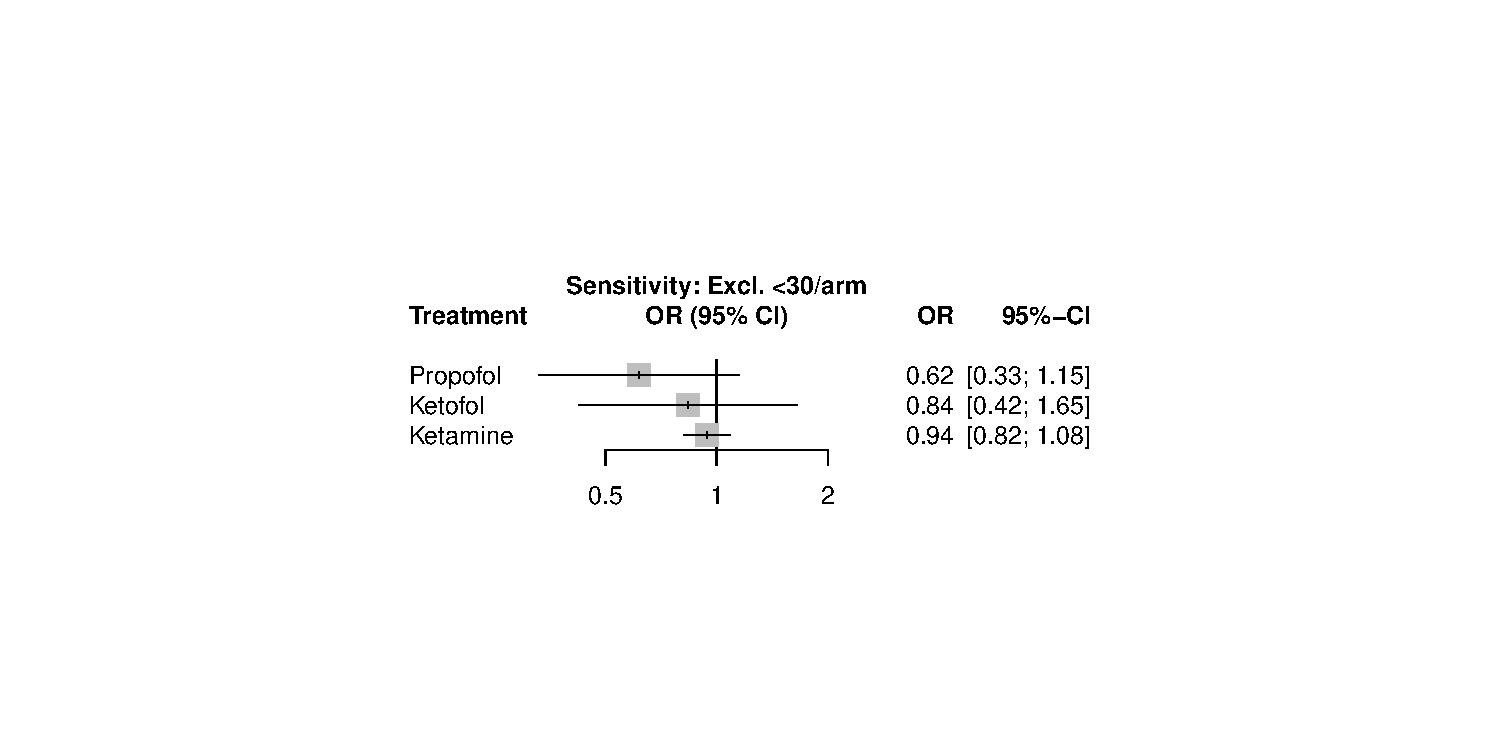
\includegraphics[width=0.85\textwidth]{eFigure14_sens_no_small.pdf}
\caption*{\textbf{eFigure~\theefigure.} Sensitivity analysis excluding small studies ($<$30 patients per arm; Cinar 2011 excluded; 8 studies remaining).}
\end{efigure}

\begin{efigure}[p]
\centering
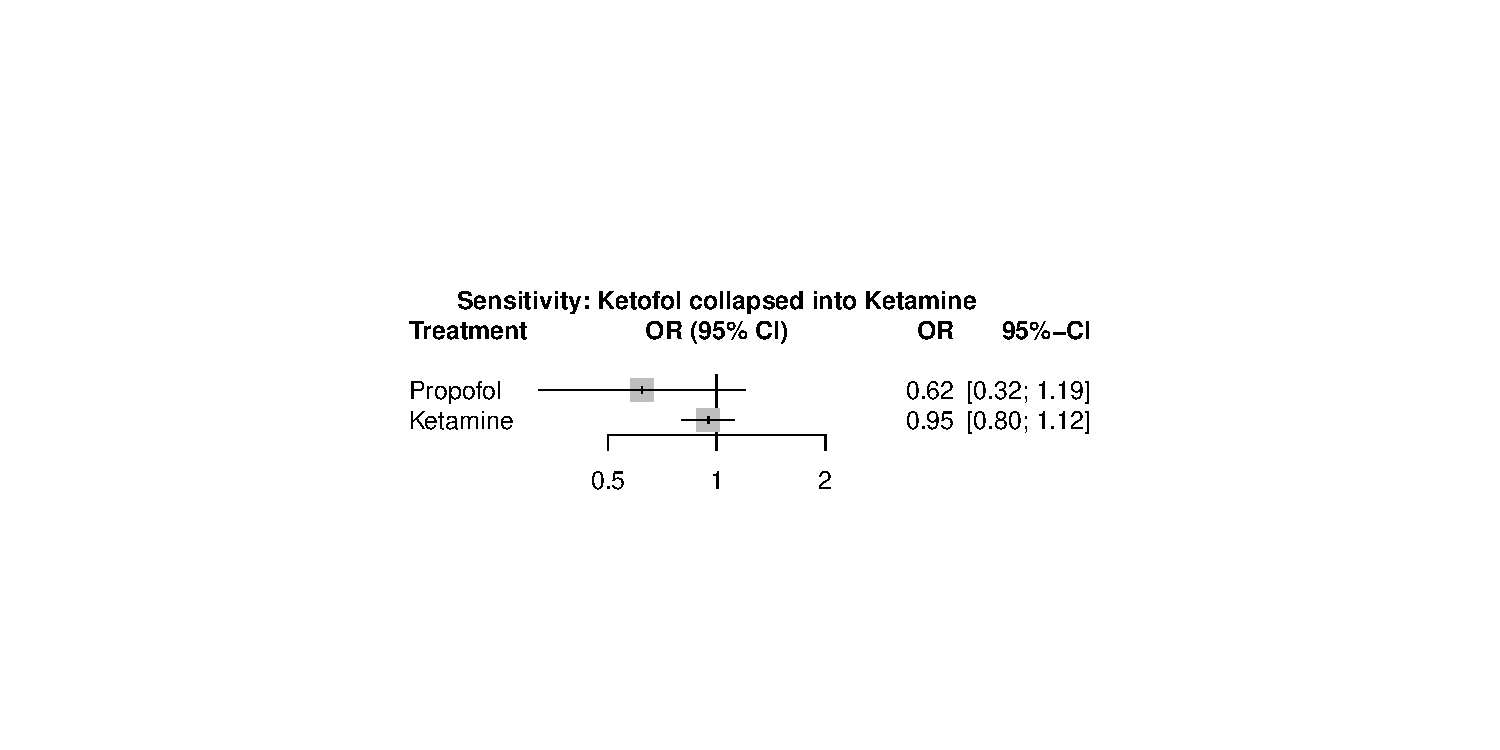
\includegraphics[width=0.85\textwidth]{eFigure15_sens_collapse_ketofol.pdf}
\caption*{\textbf{eFigure~\theefigure.} Sensitivity analysis collapsing the ketofol node into ketamine (three-node network: etomidate, ketamine, propofol).}
\end{efigure}

\begin{efigure}[p]
\centering
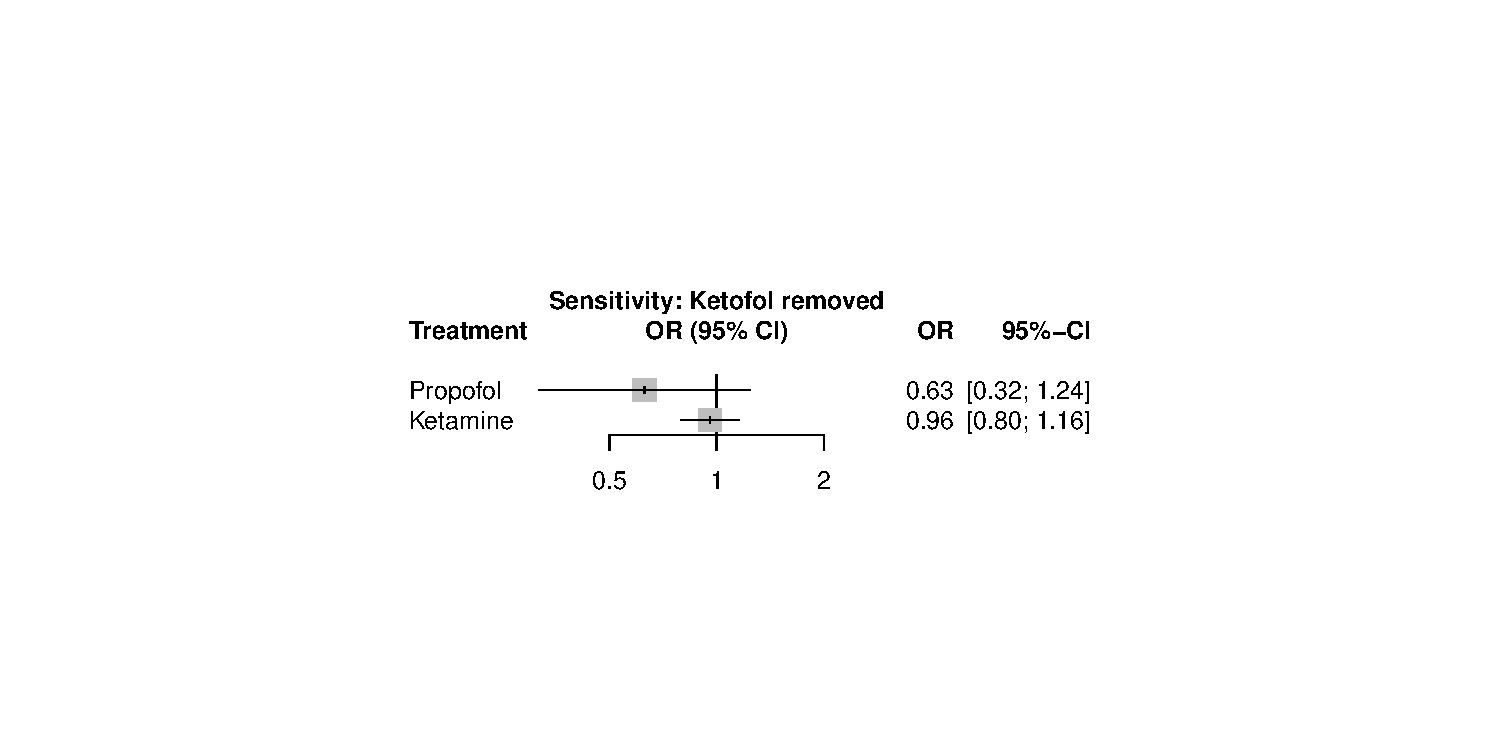
\includegraphics[width=0.85\textwidth]{eFigure16_sens_remove_ketofol.pdf}
\caption*{\textbf{eFigure~\theefigure.} Sensitivity analysis removing the ketofol node and the corresponding study (Smischney 2019 excluded; 8 studies, three-node network).}
\end{efigure}

% --- eFigures 17--21: Sensitivity excluding Casey 2025 (RSI trial) ---

\begin{efigure}[p]
\centering
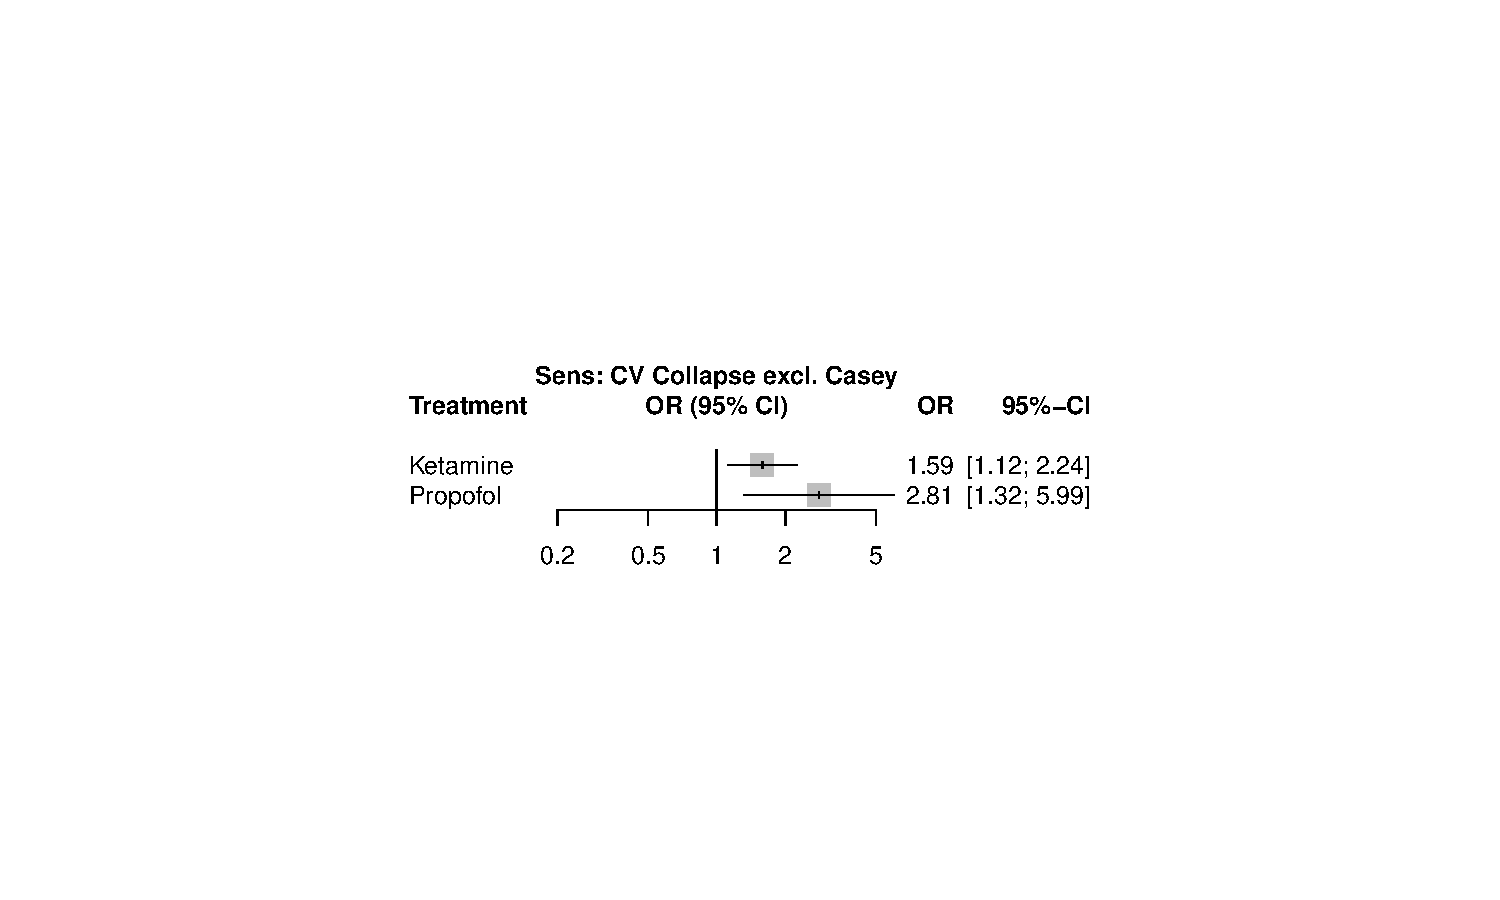
\includegraphics[width=0.85\textwidth]{eFigure17_sens_excl_casey_cv_collapse.pdf}
\caption*{\textbf{eFigure~\theefigure.} Sensitivity analysis excluding Casey 2025 (RSI trial): cardiovascular collapse. Two studies remaining (Matchett 2022, Schmidt 2025). Ketamine vs etomidate OR 1.59 (1.12--2.24); finding remains significant.}
\end{efigure}

\begin{efigure}[p]
\centering
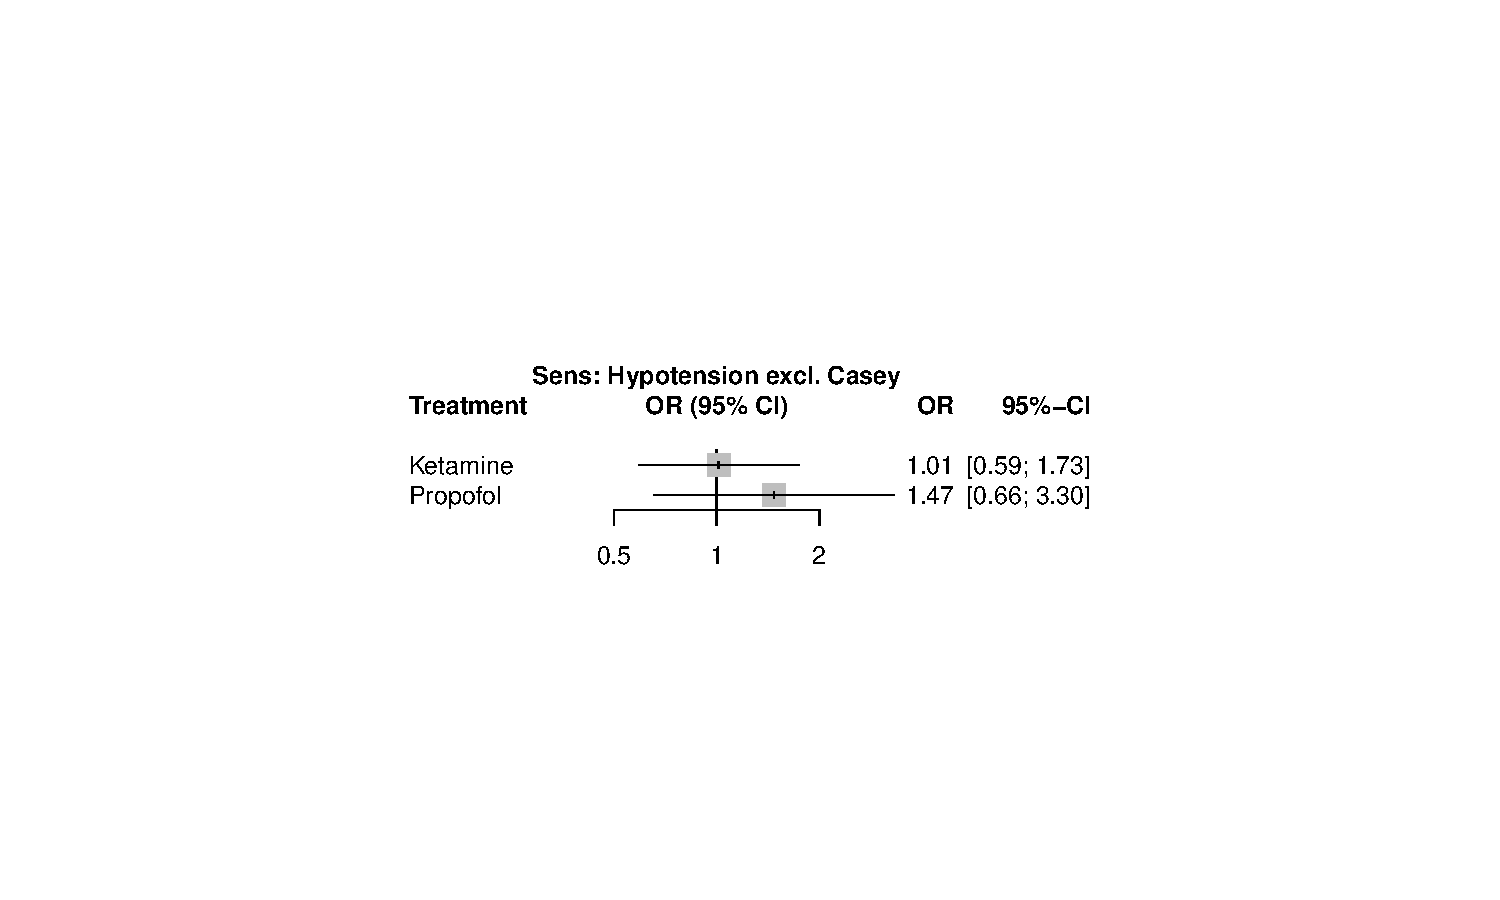
\includegraphics[width=0.85\textwidth]{eFigure18_sens_excl_casey_hypotension.pdf}
\caption*{\textbf{eFigure~\theefigure.} Sensitivity analysis excluding Casey 2025 (RSI trial): post-induction hypotension. Three studies remaining (Knack, Srivilaithon, Schmidt). Ketamine vs etomidate OR 1.01 (0.59--1.73); finding attenuated and no longer significant.}
\end{efigure}

\begin{efigure}[p]
\centering
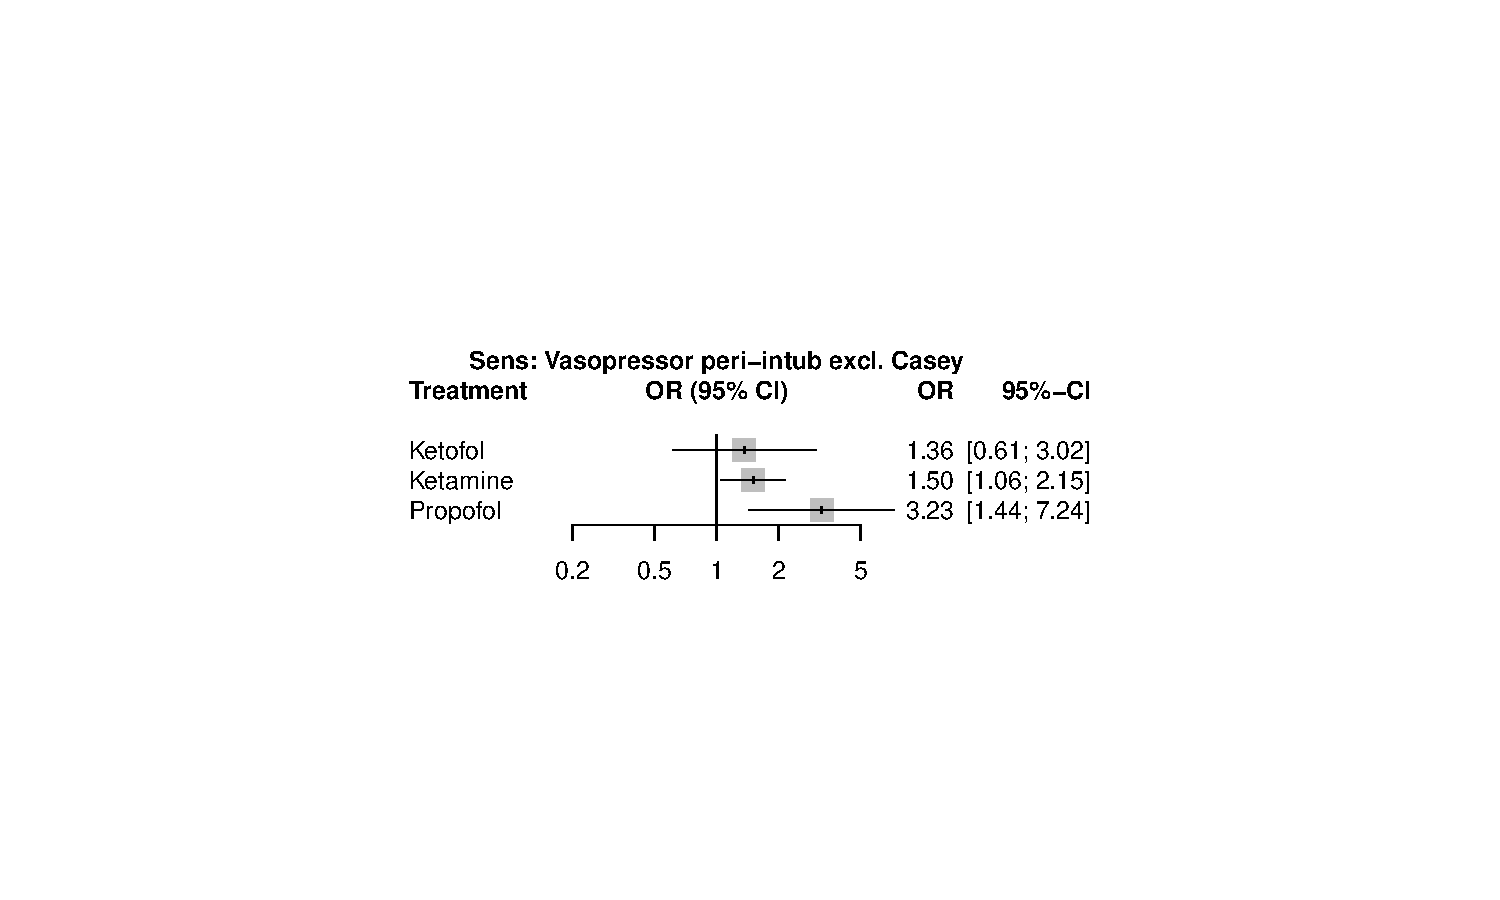
\includegraphics[width=0.85\textwidth]{eFigure19_sens_excl_casey_vaso_peri.pdf}
\caption*{\textbf{eFigure~\theefigure.} Sensitivity analysis excluding Casey 2025 (RSI trial): peri-intubation vasopressor use. Four studies remaining (Cinar, Smischney, Matchett, Schmidt). Ketamine vs etomidate OR 1.50 (1.06--2.15); finding remains significant.}
\end{efigure}

\begin{efigure}[p]
\centering
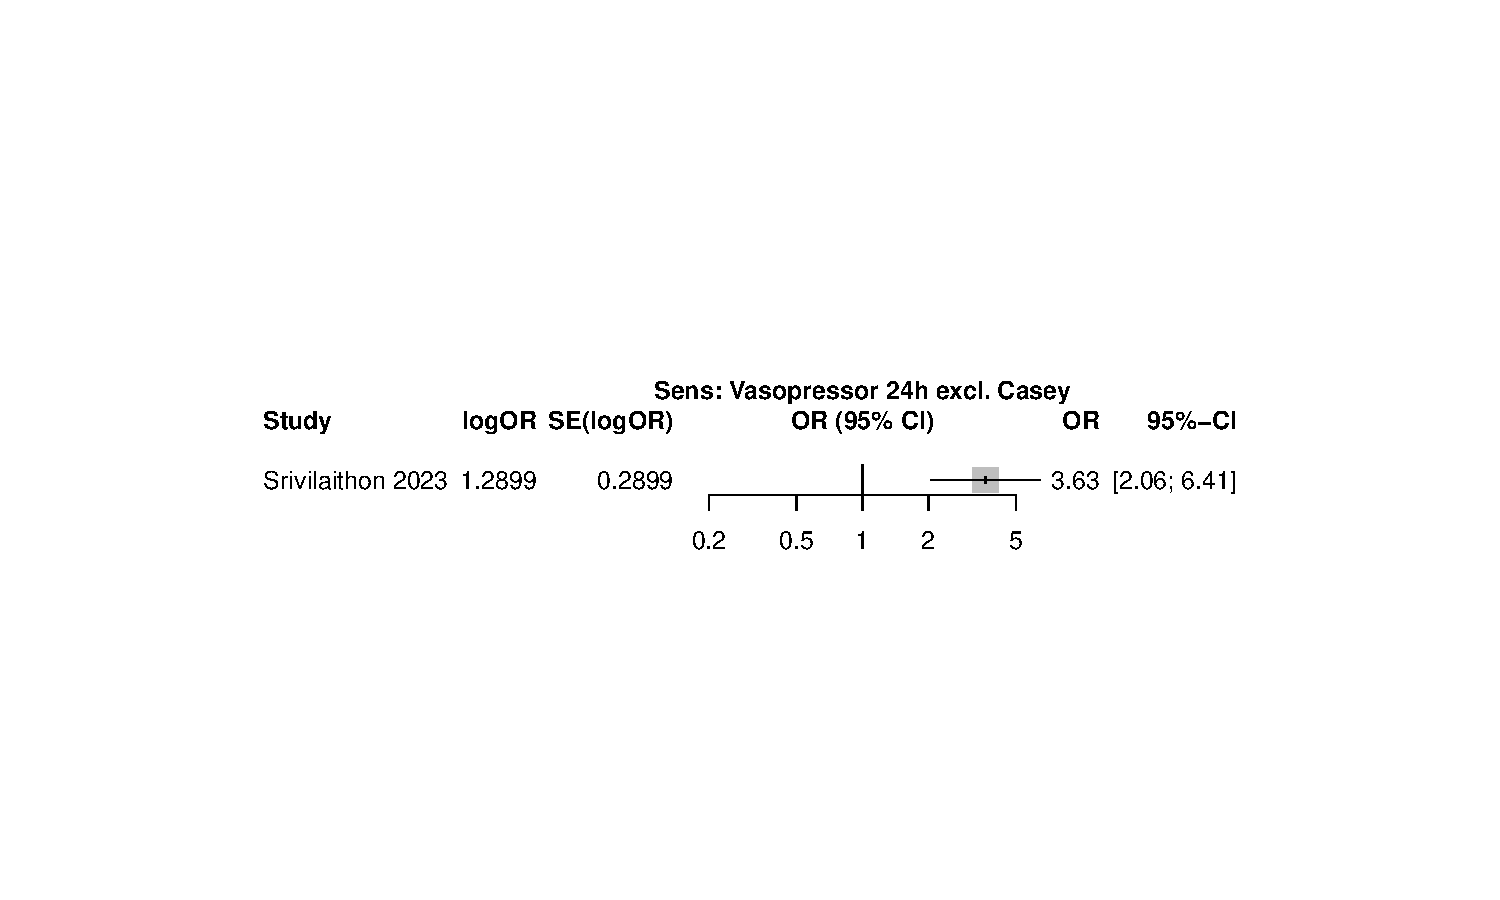
\includegraphics[width=0.85\textwidth]{eFigure20_sens_excl_casey_vaso_24h.pdf}
\caption*{\textbf{eFigure~\theefigure.} Sensitivity analysis excluding Casey 2025 (RSI trial): vasopressor use at 24 hours (etomidate vs ketamine direction). One study remaining (Srivilaithon 2023). OR 3.63 (2.06--6.41), indicating substantially higher 24-hour vasopressor use with etomidate in this sepsis-only population. Heterogeneity present in the main analysis ($I^2$ = 96\%) cannot be assessed with a single study.}
\end{efigure}

\begin{efigure}[p]
\centering
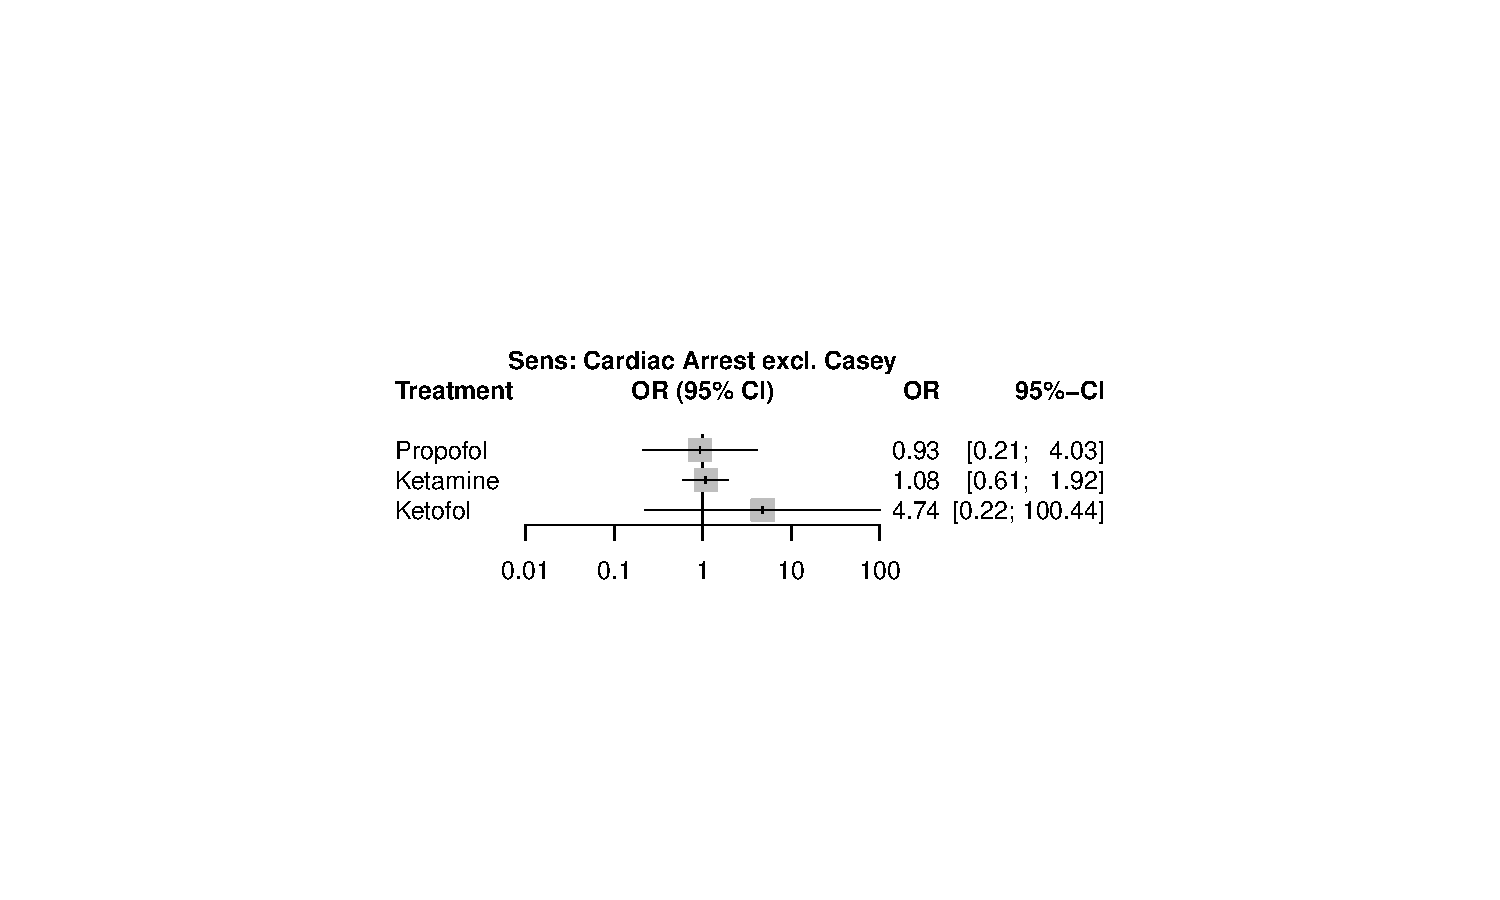
\includegraphics[width=0.85\textwidth]{eFigure21_sens_excl_casey_cardiac_arrest.pdf}
\caption*{\textbf{eFigure~\theefigure.} Sensitivity analysis excluding Casey 2025 (RSI trial): peri-intubation cardiac arrest. Six studies remaining. Ketamine vs etomidate OR 1.09 (0.60--1.95); finding unchanged.}
\end{efigure}

\clearpage

% ============================================================================
% APPENDIX C: GRADE / CINeMA ASSESSMENTS
% ============================================================================
\section{Certainty of Evidence (CINeMA Framework)}
\label{sec:grade}

Certainty of evidence was assessed using the CINeMA framework (Confidence in Network Meta-Analysis) for key comparisons.

\subsection{Primary outcome: short-term mortality}

% --- eTable 1: E vs K CINeMA ---
\begin{etabletab}[H]
\centering
\caption*{\textbf{eTable~\theetable.} CINeMA assessment --- Ketamine vs Etomidate, mortality (OR 0.96, 95\% CI 0.80--1.16)}
\small
\begin{tabularx}{\textwidth}{L{2.5cm} C{2cm} X}
\toprule
\textbf{Domain} & \textbf{Judgement} & \textbf{Rationale} \\
\midrule
Within-study bias & Some concerns & All 7 contributing studies rated ``some concerns'' (6) or ``high risk'' (1, Punt). Open-label designs in 6/7 studies, but mortality is objective and the risk-of-bias subgroup analysis showed no effect modification ($p$ = 0.88). Not downgraded. \\
Reporting bias & No concerns & 9 studies in NMA; funnel plot shows no clear asymmetry. Most studies pre-registered. \\
Indirectness & No concerns & All 7 studies directly compare E and K in the target population. Settings include ED, ICU, and mixed. \\
Imprecision & Some concerns & 95\% CI (0.80--1.16) includes OR = 1.0; on an absolute scale at 30\% baseline mortality, the CI corresponds to approximately $-$5\% to $+$4\%, which does not exclude a clinically important difference of 2--3\%. \textbf{Downgraded one level.} \\
Heterogeneity & No concerns & $I^2$ = 30\%, $\tau^2$ = 0.017. Subgroup analyses showed no significant effect modification (setting $p$ = 0.83; RoB $p$ = 0.88). \\
Incoherence & No concerns & 100\% direct evidence. \\
\midrule
\multicolumn{3}{l}{\textbf{Overall certainty: MODERATE} (downgraded one level for imprecision)} \\
\bottomrule
\end{tabularx}
\end{etabletab}

% --- eTable 2: K vs P CINeMA ---
\begin{etabletab}[H]
\centering
\caption*{\textbf{eTable~\theetable.} CINeMA assessment --- Ketamine vs Propofol, mortality (OR 1.53, 95\% CI 0.80--2.93)}
\small
\begin{tabularx}{\textwidth}{L{2.5cm} C{2cm} X}
\toprule
\textbf{Domain} & \textbf{Judgement} & \textbf{Rationale} \\
\midrule
Within-study bias & Some concerns & Based entirely on PROMINE (open-label, mITT excluding 15.5\% including pre-consent deaths). \\
Reporting bias & Some concerns & Single direct study. Mortality was not the primary endpoint of PROMINE. Cannot assess small-study effects. \\
Indirectness & Some concerns & PROMINE used esketamine 2 mg/kg in high-severity ICU population in Brazil (hospital mortality $\sim$55\%). May not generalize to ED, lower-acuity, or racemic ketamine. \\
Imprecision & Major concerns & Wide 95\% CI (0.80--2.93) spanning from meaningful benefit to substantial harm. Only 175 patients. \\
Heterogeneity & No concerns & Single study. \\
Incoherence & No concerns & 100\% direct evidence. \\
\midrule
\multicolumn{3}{l}{\textbf{Overall certainty: LOW} (downgraded for imprecision [major] and indirectness)} \\
\bottomrule
\end{tabularx}
\end{etabletab}

% --- eTable 3: E vs P CINeMA ---
\begin{etabletab}[H]
\centering
\caption*{\textbf{eTable~\theetable.} CINeMA assessment --- Etomidate vs Propofol, mortality (OR 0.63, 95\% CI 0.32--1.24; indirect)}
\small
\begin{tabularx}{\textwidth}{L{2.5cm} C{2cm} X}
\toprule
\textbf{Domain} & \textbf{Judgement} & \textbf{Rationale} \\
\midrule
Within-study bias & Some concerns & Entirely indirect: 50\% from E--K studies + 50\% from PROMINE. Contribution-weighted RoB: some concerns. \\
Reporting bias & Some concerns & Indirect comparison limits assessment. \\
Indirectness & Major concerns & No direct evidence. Transitivity assumption through ketamine node. E--K and K--P studies differ in setting, ketamine formulation (racemic vs esketamine), and population severity. \\
Imprecision & Major concerns & Wide 95\% CI (0.32--1.24). Indirect estimation amplifies uncertainty. \\
Heterogeneity & No concerns & Network-level $I^2$ = 30\%. \\
Incoherence & No concerns & Cannot assess (no direct evidence). \\
\midrule
\multicolumn{3}{l}{\textbf{Overall certainty: VERY LOW} (downgraded for bias, indirectness [major], imprecision [major])} \\
\bottomrule
\end{tabularx}
\end{etabletab}

\subsection{Key secondary outcomes (Ketamine vs Etomidate)}

% --- eTable 4: Secondary outcomes CINeMA ---
\begin{etabletab}[H]
\centering
\caption*{\textbf{eTable~\theetable.} CINeMA assessment summary --- Secondary outcomes, Ketamine vs Etomidate}
\small
\begin{tabularx}{\textwidth}{L{2.2cm} C{1.2cm} C{1.2cm} C{1.2cm} C{1.2cm} C{1.2cm} C{1.2cm} C{1.5cm}}
\toprule
\textbf{Outcome} & \textbf{Bias} & \textbf{Report.} & \textbf{Indir.} & \textbf{Imprec.} & \textbf{Heter.} & \textbf{Incoh.} & \textbf{Overall} \\
\midrule
CV collapse & SC & SC & NC & NC & NC & NC & Moderate \\
Hypotension & SC & SC & SC & NC & NC & NC & Low \\
Vaso (peri) & SC & SC & SC & NC & NC & NC & Low \\
First-pass & SC & SC & NC & NC & NC & NC & Moderate \\
Cardiac arr. & SC & SC & NC & SC & NC & NC & Low \\
\bottomrule
\end{tabularx}
\vspace{4pt}
\raggedright\footnotesize
SC = some concerns; NC = no concerns. Vaso = vasopressor use; peri = peri-intubation. CV = cardiovascular. See main text for detailed rationale.
\end{etabletab}

\newpage

% ============================================================================
% APPENDIX D: DATA EXTRACTIONS
% ============================================================================
\section{Data Extractions}
\label{sec:extractions}

Data were extracted independently by two reviewers (or by machine extraction with full human verification against source PDFs). Below we present the mortality data summary followed by full per-study extraction forms for all 9 included studies (N = 4,672 patients).

\subsection{Summary of mortality data}

\begin{table}[H]
\centering
\small
\begin{tabularx}{\textwidth}{L{2.8cm} C{0.6cm} L{2.6cm} C{0.7cm} C{1cm} C{1.4cm} C{1.4cm} C{1.4cm}}
\toprule
\textbf{Study} & \textbf{Year} & \textbf{Comparison} & \textbf{N} & \textbf{Setting} & \textbf{Timepoint} & \textbf{Arm A deaths} & \textbf{Arm B deaths} \\
\midrule
Jabre (KETASED) & 2009 & E vs K & 469 & Mixed & 28-day & 81/234 & 72/235 \\
Cinar$^{*}$ & 2011 & E vs K & 22 & ICU & ICU & 5/12 & 8/10 \\
Punt$^{*}$ & 2014 & E vs SK & 301 & ICU & 28-day & 61/161 & 54/140 \\
Smischney & 2019 & E vs KF & 152 & ICU & Hospital & 26/73 & 25/79 \\
Matchett (EvK) & 2022 & E vs K & 791 & ICU & 28-day & 142/396 & 131/395 \\
Knack & 2023 & E vs K & 143 & ED & 30-day & 15/73 & 8/70 \\
Srivilaithon & 2023 & E vs K & 260 & ED & 28-day & 25/130 & 35/130 \\
Casey (RSI) & 2025 & E vs K & 2,359 & Mixed & 28-day & 345/1186 & 330/1173 \\
Schmidt (PROMINE) & 2025 & P vs ESK & 175 & ICU & Hospital & 42/84 & 55/91 \\
\bottomrule
\end{tabularx}
\vspace{4pt}
\raggedright\footnotesize
E = etomidate; K = ketamine; SK = S-ketamine; ESK = esketamine; P = propofol; KF = ketofol. Arm A = first-named treatment; Arm B = second-named treatment.\\
$^{*}$Ketamine arm included midazolam adjunct --- flagged for sensitivity analysis.
\end{table}

\newpage

% ============================================================================
% PER-STUDY EXTRACTIONS
% ============================================================================
\subsection{Per-study extraction forms}

% -----------------------------------------------------------------------
\subsubsection{Study 1: Jabre 2009 (KETASED)}

\paragraph{Identification and design.}
Jabre P et al., \textit{The Lancet} 2009. France. KETASED trial (NCT00440102). Funded by French Ministry of Health (PHRC 2006 AOM06103). Prospective, randomized, single-blind, parallel-group trial across 12 EMS/ED centers (65 receiving ICUs). April 2007 to February 2008. Single-blind: enrolling emergency physicians aware of allocation; ICU nurses and intensivists masked.

\paragraph{Population.}

\begin{table}[H]
\centering\footnotesize
\begin{tabularx}{\textwidth}{L{4cm} C{3cm} C{3cm}}
\toprule
& \textbf{Etomidate} & \textbf{Ketamine} \\
\midrule
Randomized, n & 328 & 327 \\
Analyzed (mITT), n & 234 & 235 \\
Age, mean (SD) & 57 (18) & 59 (19) \\
Male, n (\%) & 147 (63\%) & 133 (57\%) \\
SAPS II, mean (SD) & 51.2 (18.3) & 50.5 (17.4) \\
GCS, median (range) & 6 (3--15) & 7 (3--15) \\
Baseline SBP, mean (SD) mmHg & 132 (38) & 128 (32) \\
Sepsis, n (\%) & 41 (18\%) & 35 (15\%) \\
\bottomrule
\end{tabularx}
\end{table}

\noindent\textbf{Inclusion:} Adults $\geq$18 years requiring emergency orotracheal intubation with sedation.\\
\textbf{Exclusion:} Cardiac arrest; contraindications to succinylcholine, ketamine, or etomidate; known pregnancy.\\
\textbf{mITT exclusions:} 186/655 (28\%) excluded (ICU discharge $<$3 days, pre-hospital death, consent withdrawal, missing data).

\paragraph{Interventions.}
Etomidate 0.3 mg/kg vs ketamine 2 mg/kg, both IV bolus. Succinylcholine 1 mg/kg in both arms. No co-induction agents. Post-intubation: standardized midazolam 0.1 mg/kg/h + fentanyl. Strict RSI protocol (fixed doses).

\paragraph{Outcomes.}

\begin{table}[H]
\centering\footnotesize
\begin{tabularx}{\textwidth}{L{4cm} C{2.5cm} C{2.5cm} X}
\toprule
\textbf{Outcome} & \textbf{Etomidate} & \textbf{Ketamine} & \textbf{Effect} \\
\midrule
28-day mortality & 81/234 (35\%) & 72/235 (31\%) & OR 1.2 (0.8--1.8), $p$ = 0.36 \\
Cardiac arrest (peri-intub.) & 7/234 (3\%) & 4/235 (2\%) & RD 1.3 pp \\
Change in SBP, median (IQR) & 5 ($-$11 to 30) & 10 ($-$10 to 33) & $-$5 ($-$13 to 2) \\
Catecholamine support (ICU) & 137/234 (59\%) & 120/235 (51\%) & RD 7.5 pp, $p$ = 0.10 \\
Difficult intubation (IDS $>$5) & 24 (10\%) & 20 (9\%) & --- \\
\bottomrule
\end{tabularx}
\end{table}

\paragraph{Risk of bias (RoB 2).}

\begin{table}[H]
\centering\footnotesize
\begin{tabularx}{\textwidth}{L{3cm} C{2cm} X}
\toprule
\textbf{Domain} & \textbf{Judgement} & \textbf{Support} \\
\midrule
D1: Randomization & Low risk & Computerized RNG, blocks of 4, stratified by center, sealed drug boxes. \\
D2: Deviations & Some concerns & Single-blind: emergency physicians aware; ICU staff masked. \\
D3: Missing data & Some concerns & mITT excluded 28\%. ITT (n = 650) consistent ($p$ = 0.54). \\
D4: Measurement & Low risk & 28-day mortality is objective. \\
D5: Reporting & Low risk & Pre-registered (NCT00440102). \\
\textbf{Overall} & \textbf{Some concerns} & Partial blinding + substantial mITT exclusions. \\
\bottomrule
\end{tabularx}
\end{table}

\paragraph{Notes.}
Primary endpoint was maximum SOFA score. Adrenal insufficiency significantly higher with etomidate: OR 6.7 (95\% CI 3.5--12.7). Prehospital enrollment (EMS setting). For NMA: 81/234 (etomidate) vs 72/235 (ketamine).

\bigskip

% -----------------------------------------------------------------------
\subsubsection{Study 2: Cinar 2011}

\paragraph{Identification and design.}
Cinar O et al., \textit{J Turkish Soc Intensive Care} 2011. Turkey. No trial registration. Single-center (Baskent University Hospital, Ankara). Double-blind RCT: identical syringes prepared by uninvolved clinician; all intubations by single operator. Ethics approval KA09/27.

\paragraph{Population.}

\begin{table}[H]
\centering\footnotesize
\begin{tabularx}{\textwidth}{L{4cm} C{3cm} C{3cm}}
\toprule
& \textbf{Etomidate} & \textbf{Ketamine + Midazolam} \\
\midrule
Analyzed, n & 12 & 10 \\
Age, mean $\pm$ SD & 63.8 $\pm$ 20.3 & 72.5 $\pm$ 7.8 \\
Female, n (\%) & 7 (58\%) & 4 (40\%) \\
APACHE II, mean $\pm$ SD & 28.7 $\pm$ 5.4 & 32.1 $\pm$ 7.0 \\
\bottomrule
\end{tabularx}
\end{table}

\noindent\textbf{Inclusion:} ICU patients requiring emergency intubation (GCS $<$8, respiratory failure).\\
\textbf{Exclusion:} Cardiac arrest; prior corticosteroids; adrenal insufficiency; psychotic disorder.

\paragraph{Interventions.}
Etomidate 0.3 mg/kg vs ketamine 2 mg/kg + midazolam 0.03 mg/kg (combined in same syringe), both IV. No NMBA used in either arm. All intubations by same operator. Strict protocol.

\paragraph{Outcomes.}

\begin{table}[H]
\centering\footnotesize
\begin{tabularx}{\textwidth}{L{4cm} C{2.5cm} C{2.5cm} X}
\toprule
\textbf{Outcome} & \textbf{Etomidate} & \textbf{Ket + Midaz} & \textbf{Effect} \\
\midrule
ICU mortality & 5/12 (42\%) & 8/10 (80\%) & $p$ = 0.099 \\
Vasopressor (peri-intub.) & 2/12 (17\%) & 2/10 (20\%) & $p$ = 1.0 \\
Cardiac arrest (peri-intub.) & 1/12 & 1/10 & --- \\
\bottomrule
\end{tabularx}
\end{table}

\paragraph{Risk of bias (RoB 2).}

\begin{table}[H]
\centering\footnotesize
\begin{tabularx}{\textwidth}{L{3cm} C{2cm} X}
\toprule
\textbf{Domain} & \textbf{Judgement} & \textbf{Support} \\
\midrule
D1: Randomization & Some concerns & Web-based RNG. Very small sample; APACHE II imbalance. \\
D2: Deviations & Low risk & Double-blind (identical syringes, single operator). \\
D3: Missing data & Low risk & All 22 accounted for. \\
D4: Measurement & Low risk & Mortality is objective. \\
D5: Reporting & Some concerns & No trial registration. Mortality was secondary. \\
\textbf{Overall} & \textbf{Some concerns} & Small unregistered trial. Double-blind is a strength. \\
\bottomrule
\end{tabularx}
\end{table}

\paragraph{Notes.}
\textbf{Flagged for sensitivity analysis:} ketamine arm received midazolam adjunct. Extremely small trial (n = 22). No NMBA used. ICU mortality (only available timepoint). For NMA: 5/12 (etomidate) vs 8/10 (ketamine).

\bigskip

% -----------------------------------------------------------------------
\subsubsection{Study 3: Punt 2014}

\paragraph{Identification and design.}
Punt CD, Dormans TPJ et al., \textit{Neth J Crit Care} 2014. The Netherlands. ISRCTN39347168. Single-center cluster-randomized trial (Atrium Medical Centre, Heerlen; 3 ICU units, 21 beds). Open-label. April 2008 to end of 2009. Cluster design: 2 units used etomidate and 1 used S-ketamine for 10 months, then reversed.

\paragraph{Population.}

\begin{table}[H]
\centering\footnotesize
\begin{tabularx}{\textwidth}{L{4cm} C{3cm} C{3cm}}
\toprule
& \textbf{Etomidate} & \textbf{S-ketamine + Midazolam} \\
\midrule
Analyzed, n & 161 & 140 \\
Age, mean (SD) & 66 (14) & 67 (13) \\
Male, n (\%) & 95 (59\%) & 89 (64\%) \\
APACHE II, mean (SD) & 25 (7) & 24 (7) \\
Sepsis, n & 58 & 54 \\
\bottomrule
\end{tabularx}
\end{table}

\noindent\textbf{Inclusion:} All critically ill adults intubated in participating ICU units.\\
\textbf{Exclusion:} Already intubated before ICU admission; received etomidate $<$72h before enrollment.

\paragraph{Interventions.}
Etomidate 0.2--0.3 mg/kg vs S-ketamine 0.5 mg/kg + midazolam 2.5 mg, both IV. Rocuronium in both arms. Pragmatic protocol.

\paragraph{Outcomes.}

\begin{table}[H]
\centering\footnotesize
\begin{tabularx}{\textwidth}{L{4cm} C{2.5cm} C{2.5cm} X}
\toprule
\textbf{Outcome} & \textbf{Etomidate} & \textbf{S-ket + Midaz} & \textbf{Effect} \\
\midrule
28-day mortality & 61/161 (38\%) & 54/140 (39\%) & $p$ = 0.998 \\
NE hours (72h), mean (SD) & 26 (31) & 29 (29) & $p$ = 0.389 \\
ICU LOS, days, mean (SD) & 16 (25) & 19 (27) & $p$ = 0.318 \\
\bottomrule
\end{tabularx}
\end{table}

\paragraph{Risk of bias (RoB 2).}

\begin{table}[H]
\centering\footnotesize
\begin{tabularx}{\textwidth}{L{3cm} C{2cm} X}
\toprule
\textbf{Domain} & \textbf{Judgement} & \textbf{Support} \\
\midrule
D1: Randomization & High risk & Cluster-randomized by ICU unit; allocation predictable. \\
D2: Deviations & Some concerns & Open-label. Midazolam only in S-ketamine arm. \\
D3: Missing data & Low risk & 301 analyzed with clear accounting. \\
D4: Measurement & Low risk & 28-day mortality is objective. \\
D5: Reporting & Low risk & Registered (ISRCTN39347168). Mortality was primary. \\
\textbf{Overall} & \textbf{High risk} & Cluster design without individual concealment; systematic co-intervention difference. \\
\bottomrule
\end{tabularx}
\end{table}

\paragraph{Notes.}
\textbf{Flagged for sensitivity analysis:} S-ketamine arm received midazolam 2.5 mg. S-ketamine mapped to Ketamine node. Cluster-randomized design is a major limitation. For NMA: 61/161 (etomidate) vs 54/140 (S-ketamine).

\bigskip

% -----------------------------------------------------------------------
\subsubsection{Study 4: Smischney 2019 (KEEP PACE)}

\paragraph{Identification and design.}
Smischney NJ et al., \textit{J Trauma Acute Care Surg} 2019. United States. KEEP PACE trial (NCT02105415). Funded by Dept of Anesthesiology, Mayo Clinic; CTSA grant. Single-center (Mayo Clinic, Rochester, MN). Open-label intervention; outcome adjudicators and statistician blinded. July 2014 to October 2017.

\paragraph{Population.}

\begin{table}[H]
\centering\footnotesize
\begin{tabularx}{\textwidth}{L{4cm} C{3cm} C{3cm}}
\toprule
& \textbf{Etomidate} & \textbf{Ketofol} \\
\midrule
Randomized, n & 76 & 84 \\
Analyzed, n & 73 & 79 \\
Age, mean $\pm$ SD & 60.0 $\pm$ 18.3 & 62.1 $\pm$ 17.2 \\
Male, n (\%) & 38 (52\%) & 48 (61\%) \\
APACHE III, mean $\pm$ SD & 86.7 $\pm$ 30.4 & 85.8 $\pm$ 31.3 \\
Baseline MAP, mean $\pm$ SD mmHg & 82.8 $\pm$ 17.9 & 80.9 $\pm$ 13.3 \\
On vasopressors, n (\%) & 21 (29\%) & 17 (22\%) \\
Sepsis, n (\%) & 57 (78\%) & 61 (77\%) \\
\bottomrule
\end{tabularx}
\end{table}

\noindent\textbf{Inclusion:} Adults $\geq$18 years admitted to ICU requiring emergent intubation.\\
\textbf{Exclusion:} Cardiac arrest; ICP pathology; chronic opioid dependence; bipolar/schizophrenia; egg allergy; weight $>$140 or $<$30 kg.

\paragraph{Interventions.}
Etomidate 0.15 mg/kg (reduced dose) vs ketofol (ketamine 0.5 mg/kg + propofol 0.5 mg/kg, single syringe). Fentanyl 50 $\mu$g IV standard in both arms. Rescue doses allowed. Succinylcholine or rocuronium per clinician choice. Pragmatic protocol.

\paragraph{Outcomes.}

\begin{table}[H]
\centering\footnotesize
\begin{tabularx}{\textwidth}{L{4cm} C{2.5cm} C{2.5cm} X}
\toprule
\textbf{Outcome} & \textbf{Etomidate} & \textbf{Ketofol} & \textbf{Effect} \\
\midrule
Hospital mortality & 26/73 (36\%) & 25/79 (32\%) & $p$ = 0.605 \\
Vasopressor 5 min & 13/73 (18\%) & 18/79 (24\%) & $p$ = 0.446 \\
Vasopressor 15 min--24h & 57/73 (78\%) & 64/79 (81\%) & $p$ = 0.691 \\
Adrenal insuff. 3--5h & 13/16 (81\%) & 5/13 (38\%) & $p$ = 0.027 \\
\bottomrule
\end{tabularx}
\end{table}

\paragraph{Risk of bias (RoB 2).}

\begin{table}[H]
\centering\footnotesize
\begin{tabularx}{\textwidth}{L{3cm} C{2cm} X}
\toprule
\textbf{Domain} & \textbf{Judgement} & \textbf{Support} \\
\midrule
D1: Randomization & Low risk & Computer-generated, stratified by unit and shock, sealed envelopes. \\
D2: Deviations & Some concerns & Open-label. Co-interventions noncontrolled. \\
D3: Missing data & Low risk & 8/160 (5\%) withdrew consent. 152 analyzed. \\
D4: Measurement & Low risk & Hospital mortality is objective. \\
D5: Reporting & Low risk & Pre-registered (NCT02105415). DSMB oversight. \\
\textbf{Overall} & \textbf{Some concerns} & Open-label with noncontrolled co-interventions. \\
\bottomrule
\end{tabularx}
\end{table}

\paragraph{Notes.}
Only trial providing the \textbf{ketofol--etomidate} edge in the NMA. Both drug doses reduced from standard. Primary endpoint was MAP at 5 min. For NMA: 26/73 (etomidate) vs 25/79 (ketofol).

\bigskip

% -----------------------------------------------------------------------
\subsubsection{Study 5: Matchett 2022 (EvK)}

\paragraph{Identification and design.}
Matchett G et al., \textit{Intensive Care Med} 2022. United States. EvK trial (NCT02643381). EFIC trial at UT-Southwestern Medical Center, Dallas. Single-center, open-label RCT. June 2016 to September 2020. No external funding.

\paragraph{Population.}

\begin{table}[H]
\centering\footnotesize
\begin{tabularx}{\textwidth}{L{4cm} C{3cm} C{3cm}}
\toprule
& \textbf{Etomidate} & \textbf{Ketamine} \\
\midrule
Randomized, n & 400 & 401 \\
Analyzed, n & 396 & 395 \\
Age, mean (SD) & 55.8 (15.2) & 55.4 (16) \\
Female, n (\%) & 153 (38.6\%) & 150 (38\%) \\
Indication: shock, n (\%) & 189 (47.7\%) & 174 (44.1\%) \\
Baseline SBP, mean (SD) mmHg & 120.7 (32.2) & 120.3 (29.5) \\
Sepsis, n (\%) & 136 (34.3\%) & 136 (34.4\%) \\
\bottomrule
\end{tabularx}
\end{table}

\noindent\textbf{Inclusion:} Adults $\geq$18 years requiring emergency endotracheal intubation.\\
\textbf{Exclusion:} Cardiac arrest; pregnant; previously enrolled; known allergy.

\paragraph{Interventions.}
Etomidate 0.2--0.3 mg/kg (median actual 0.2 mg/kg) vs ketamine 1--2 mg/kg (median actual 1.1 mg/kg). Rocuronium (~80\%) or succinylcholine (~18\%). Semi-standardized airway bundle protocol.

\paragraph{Outcomes.}

\begin{table}[H]
\centering\footnotesize
\begin{tabularx}{\textwidth}{L{4cm} C{2.5cm} C{2.5cm} X}
\toprule
\textbf{Outcome} & \textbf{Etomidate} & \textbf{Ketamine} & \textbf{Effect} \\
\midrule
Day 28 mortality & 142/396 (35.9\%) & 131/395 (33.2\%) & RD $-$2.7 pp ($-$9.3 to 3.9) \\
Day 7 mortality & 90/396 (22.7\%) & 59/395 (14.9\%) & RD $-$7.8 pp ($-$13 to $-$2.4)$^{\dag}$ \\
CV collapse & 69/396 (17.4\%) & 99/395 (25.1\%) & RD $-$7.6 pp ($-$13 to $-$2) \\
First-pass success & 357/391 (91.3\%) & 355/389 (91.3\%) & RD 0 pp \\
Vasopressor Days 1--4 & 235/396 (59.3\%) & 213/395 (53.9\%) & RD 5.4 pp ($-$1.5 to 12.3) \\
Cardiac arrest (post-induction CPR)$^{\ddag}$ & 13/345 (3.8\%) & 18/354 (5.1\%) & --- \\
Vasopressor bolus (peri-intubation)$^{\ddag}$ & 65/345 (18.8\%) & 92/354 (26.0\%) & --- \\
\bottomrule
\end{tabularx}
\vspace{2pt}\raggedright\footnotesize $^{\dag}$Day 7 was the original primary endpoint; significantly favored ketamine.\\
$^{\ddag}$Denominators reduced (345/354) due to $\sim$12\% missing data from nurses' code sheets (unavailable for 51 etomidate, 41 ketamine patients).
\end{table}

\paragraph{Risk of bias (RoB 2).}

\begin{table}[H]
\centering\footnotesize
\begin{tabularx}{\textwidth}{L{3cm} C{2cm} X}
\toprule
\textbf{Domain} & \textbf{Judgement} & \textbf{Support} \\
\midrule
D1: Randomization & Low risk & Computer-generated, blocks of 8, sealed envelopes. \\
D2: Deviations & Some concerns & Completely open-label. \\
D3: Missing data & Low risk & 10/801 (1.2\%) withdrawals. \\
D4: Measurement & Low risk & Day 28 mortality is objective. \\
D5: Reporting & Low risk & Pre-registered. SAP finalized before analysis. \\
\textbf{Overall} & \textbf{Some concerns} & Due to open-label design. \\
\bottomrule
\end{tabularx}
\end{table}

\paragraph{Notes.}
CV collapse higher with ketamine (25.1\% vs 17.4\%), consistent with Casey 2025. Low actual ketamine dose (median 1.1 mg/kg). Trial closed early by DSMB. For NMA: 142/396 (etomidate) vs 131/395 (ketamine).

\bigskip

% -----------------------------------------------------------------------
\subsubsection{Study 6: Knack 2023}

\paragraph{Identification and design.}
Knack SKS et al., \textit{J Emerg Med} 2023. United States. NCT01823328. EFIC trial at Hennepin County Medical Center, Minneapolis. Single-center, partially blinded (ED team aware; ICU team blinded). September 2013 to November 2015. Full publication of Driver 2014 conference abstract.

\paragraph{Population.}

\begin{table}[H]
\centering\footnotesize
\begin{tabularx}{\textwidth}{L{4cm} C{3cm} C{3cm}}
\toprule
& \textbf{Etomidate} & \textbf{Ketamine} \\
\midrule
Analyzed (ITT), n & 73 & 70 \\
Age, median (IQR) & 49 (31--58) & 50 (32--65) \\
Male, n (\%) & 49 (67\%) & 42 (60\%) \\
GCS, median (IQR) & 8 (6--11) & 7 (6--12) \\
Baseline SBP, median (IQR) & 140 (119--167) & 139 (128--161) \\
Sepsis, n (\%) & 19 (26\%) & 10 (14\%) \\
\bottomrule
\end{tabularx}
\end{table}

\noindent\textbf{Inclusion:} Adults $\geq$18 years undergoing RSI in the ED, critically ill.\\
\textbf{Exclusion:} Increased HR/BP hazardous; suspected elevated ICP; known allergy.

\paragraph{Interventions.}
Etomidate 0.3 mg/kg vs ketamine 2 mg/kg. Succinylcholine in $\sim$90\%. Pragmatic protocol (devices at physician discretion).

\paragraph{Outcomes.}

\begin{table}[H]
\centering\footnotesize
\begin{tabularx}{\textwidth}{L{4cm} C{2.5cm} C{2.5cm} X}
\toprule
\textbf{Outcome} & \textbf{Etomidate} & \textbf{Ketamine} & \textbf{Effect} \\
\midrule
30-day mortality & 15/73 (21\%) & 8/70 (11\%) & RD $-$9 pp ($-$21 to 3) \\
Hypotension (SBP $<$90) in ED & 19/72 (26\%) & 19/67 (28\%) & RD 2 pp ($-$13 to 17) \\
First-pass success & 65/73 (89\%) & 66/70 (94\%) & RD 5 pp ($-$4 to 13) \\
\bottomrule
\end{tabularx}
\end{table}

\paragraph{Risk of bias (RoB 2).}

\begin{table}[H]
\centering\footnotesize
\begin{tabularx}{\textwidth}{L{3cm} C{2cm} X}
\toprule
\textbf{Domain} & \textbf{Judgement} & \textbf{Support} \\
\midrule
D1: Randomization & Low risk & Computer-generated, permuted blocks, sealed opaque envelopes. \\
D2: Deviations & Some concerns & ED unblinded; ICU blinded. 5 crossovers. \\
D3: Missing data & Low risk & All 143 in ITT analysis. \\
D4: Measurement & Low risk & 30-day mortality is objective. \\
D5: Reporting & Some concerns & Primary outcome changed mid-trial (from mortality to max SOFA). \\
\textbf{Overall} & \textbf{Some concerns} & Partially blinded; endpoint changed mid-trial. \\
\bottomrule
\end{tabularx}
\end{table}

\paragraph{Notes.}
Small trial (N = 143). Young cohort (median age 50). 10\% absolute mortality difference (not significant). For NMA: 15/73 (etomidate) vs 8/70 (ketamine).

\bigskip

% -----------------------------------------------------------------------
\subsubsection{Study 7: Srivilaithon 2023}

\paragraph{Identification and design.}
Srivilaithon W et al., \textit{Scientific Reports} 2023. Thailand. TCTR20210213001 (Thai registry, \textbf{retrospectively registered}). Single-center (Thammasat University Hospital). Single-blind: enrolling physician aware but was not the intubating physician; outcome assessors blinded. March 2019 to December 2020.

\paragraph{Population.}

\begin{table}[H]
\centering\footnotesize
\begin{tabularx}{\textwidth}{L{4cm} C{3cm} C{3cm}}
\toprule
& \textbf{Etomidate} & \textbf{Ketamine} \\
\midrule
Analyzed, n & 130 & 130 \\
Age, mean (SD) & 73.2 (12.6) & 70.5 (14.9) \\
Male, n (\%) & 77 (59.2\%) & 76 (58.5\%) \\
qSOFA, mean (SD) & 2.2 (0.4) & 2.1 (0.3) \\
Baseline SBP, mean (SD) mmHg & 112.9 (30.7) & 118.1 (32.5) \\
Lactate, median (IQR) mmol/L & 3.6 (2.4--7.6) & 3.2 (2.2--5.4) \\
Sepsis, n (\%) & 130 (100\%) & 130 (100\%) \\
\bottomrule
\end{tabularx}
\end{table}

\noindent\textbf{Inclusion:} Adults $\geq$18 years with suspected sepsis (Sepsis-3) requiring emergency intubation in the ED.\\
\textbf{Exclusion:} Cardiac arrest; DNR; adrenal insufficiency; severe hypertension; elevated ICP.

\paragraph{Interventions.}
Etomidate 0.2--0.3 mg/kg vs ketamine 1--2 mg/kg. Succinylcholine 1.5 mg/kg (NMBA use: 65\% E vs 77\% K, $p$ = 0.04). Semi-standardized protocol.

\paragraph{Outcomes.}

\begin{table}[H]
\centering\footnotesize
\begin{tabularx}{\textwidth}{L{4cm} C{2.5cm} C{2.5cm} X}
\toprule
\textbf{Outcome} & \textbf{Etomidate} & \textbf{Ketamine} & \textbf{Effect} \\
\midrule
28-day mortality & 25/130 (19.2\%) & 35/130 (26.9\%) & RD 7.7 pp ($-$2.5 to 17.9) \\
Cardiac arrest (peri-intub.) & 2/130 (1.5\%) & 2/130 (1.5\%) & $p$ = 1.0 \\
Hypotension (SBP $<$90 / MAP $<$65) & 15/130 (11.5\%) & 14/130 (10.8\%) & RD 0.7 pp \\
Vasopressor use 24h & 57/130 (43.9\%) & 23/130 (17.7\%) & RD 26.2 pp, $p < 0.001$ \\
First-pass success & 116/130 (89.2\%) & 114/130 (87.7\%) & $p$ = 0.846 \\
\bottomrule
\end{tabularx}
\end{table}

\paragraph{Risk of bias (RoB 2).}

\begin{table}[H]
\centering\footnotesize
\begin{tabularx}{\textwidth}{L{3cm} C{2cm} X}
\toprule
\textbf{Domain} & \textbf{Judgement} & \textbf{Support} \\
\midrule
D1: Randomization & Low risk & Computer-generated, blocks of 4, sealed envelopes. \\
D2: Deviations & Some concerns & Single-blind. NMBA use differed ($p$ = 0.04). \\
D3: Missing data & Low risk & All 260 analyzed, 0 lost. \\
D4: Measurement & Low risk & 28-day mortality is objective. \\
D5: Reporting & Some concerns & Retrospectively registered (Feb 2021; trial 2019--2020). \\
\textbf{Overall} & \textbf{Some concerns} & Single-blind with differential NMBA use; retrospective registration. \\
\bottomrule
\end{tabularx}
\end{table}

\paragraph{Notes.}
Sepsis-only population (100\%). Elderly (mean age $\sim$72). Vasopressor 24h much higher with etomidate (44\% vs 18\%, $p < 0.001$) --- likely reflects adrenal suppression. For NMA: 25/130 (etomidate) vs 35/130 (ketamine).

\bigskip

% -----------------------------------------------------------------------
\subsubsection{Study 8: Casey 2025 (RSI Trial)}

\paragraph{Identification and design.}
Casey JD et al., \textit{New Engl J Med} 2025. United States. RSI trial (NCT05277896). Funded by PCORI and NHLBI. Pragmatic, multicenter, unblinded RCT. 14 sites (6 EDs + 8 ICUs) in 6 medical centers. EFIC trial. April 2022 to August 2025.

\paragraph{Population.}

\begin{table}[H]
\centering\footnotesize
\begin{tabularx}{\textwidth}{L{4cm} C{3cm} C{3cm}}
\toprule
& \textbf{Etomidate} & \textbf{Ketamine} \\
\midrule
Randomized, n & 1,189 & 1,176 \\
Analyzed, n & 1,186 & 1,173 \\
Age, median (IQR) & 60 (44--69) & 60 (45--69) \\
Female, n (\%) & 492 (41.4\%) & 498 (42.3\%) \\
APACHE II, median (IQR) & 18 (13--24) & 18 (13--24) \\
SBP at induction, median (IQR) & 127 (110--148) & 127 (110--147) \\
On vasopressors, n (\%) & 274 (23.0\%) & 246 (20.9\%) \\
Sepsis/septic shock, n (\%) & 565 (47.5\%) & 539 (45.8\%) \\
Location --- ED, n (\%) & 655 (55.1\%) & 663 (56.4\%) \\
\bottomrule
\end{tabularx}
\end{table}

\noindent\textbf{Inclusion:} Adults $\geq$18 years, critically ill, undergoing tracheal intubation with anesthesia induction.\\
\textbf{Exclusion:} Pregnant; prisoners; primary trauma; clinician determined specific agent necessary.

\paragraph{Interventions.}
Etomidate 0.2--0.3 mg/kg (median 0.28) vs ketamine 1.0--2.0 mg/kg (median 1.6), dose at clinician choice. Rocuronium ($\sim$69\%) or succinylcholine ($\sim$31\%). Pragmatic protocol.

\paragraph{Outcomes.}

\begin{table}[H]
\centering\footnotesize
\begin{tabularx}{\textwidth}{L{4cm} C{2.5cm} C{2.5cm} X}
\toprule
\textbf{Outcome} & \textbf{Etomidate} & \textbf{Ketamine} & \textbf{Effect} \\
\midrule
In-hospital death by 28d & 345/1186 (29.1\%) & 330/1173 (28.1\%) & adj.\ RD $-$0.8 pp ($-$4.5 to 2.9) \\
CV collapse & 202/1189 (17.0\%) & 260/1176 (22.1\%) & RD 5.1 pp (1.9 to 8.3) \\
\quad SBP $<$65 & 64 (5.5\%) & 73 (6.4\%) & --- \\
\quad New/incr.\ vasopressor & 189 (15.9\%) & 251 (21.3\%) & RD 5.4 pp (2.3 to 8.6) \\
\quad Cardiac arrest & 10 (0.8\%) & 12 (1.0\%) & --- \\
Hypotension (SBP $<$80) & 123/$\sim$1159 (10.6\%) & 164/$\sim$1138 (14.4\%) & RD 3.8 pp (1.1 to 6.5) \\
Vaso peri-intub. & 189/1189 (15.9\%) & 251/1176 (21.3\%) & RD 5.4 pp (2.3 to 8.6) \\
Vaso at 24h & 458/$\sim$1082 (42.3\%) & 420/$\sim$1079 (38.9\%) & RD $-$3.4 ($-$7.5 to 0.7) \\
First-pass success & 1029/$\sim$1187 (86.7\%) & 1005/$\sim$1173 (85.7\%) & RD $-$1.0 pp \\
\bottomrule
\end{tabularx}
\end{table}

\paragraph{Risk of bias (RoB 2).}

\begin{table}[H]
\centering\footnotesize
\begin{tabularx}{\textwidth}{L{3cm} C{2cm} X}
\toprule
\textbf{Domain} & \textbf{Judgement} & \textbf{Support} \\
\midrule
D1: Randomization & Low risk & Permuted blocks, stratified by site, concealed envelopes. \\
D2: Deviations & Some concerns & Unblinded. Adherence $>$99\%. Could influence co-interventions. \\
D3: Missing data & Low risk & Only 6/2,365 (0.3\%) withdrew. \\
D4: Measurement & Low risk & Mortality is objective. \\
D5: Reporting & Low risk & Pre-registered. Protocol and SAP published before analysis. \\
\textbf{Overall} & \textbf{Some concerns} & Open-label. Mortality unlikely influenced by lack of blinding. \\
\bottomrule
\end{tabularx}
\end{table}

\paragraph{Notes.}
Largest trial (N = 2,365; $\sim$48\% of total sample). CV collapse higher with ketamine (22.1\% vs 17.0\%), driven by vasopressor escalation. 24h vasopressor trend reversed (favoring ketamine). Ventricular tachycardia (post hoc): K 1.0\% vs E 0.2\%. For NMA: 345/1186 (etomidate) vs 330/1173 (ketamine).

\bigskip

% -----------------------------------------------------------------------
\subsubsection{Study 9: Schmidt 2025 (PROMINE)}

\paragraph{Identification and design.}
Schmidt RC et al., \textit{Under review} 2025. Brazil. PROMINE trial (NCT05092152). Funded by CNPq; esketamine and propofol provided by Crist\'{a}lia. Investigator-initiated, randomized, open-label, parallel-group. 2 hospitals (8 ICUs, 93 beds). Outcome assessors, data collectors, and statisticians blinded. October 2021 to October 2023.

\paragraph{Population.}

\begin{table}[H]
\centering\footnotesize
\begin{tabularx}{\textwidth}{L{4cm} C{3cm} C{3cm}}
\toprule
& \textbf{Propofol} & \textbf{Esketamine} \\
\midrule
Randomized, n & 102 & 105 \\
Analyzed (mITT), n & 84 & 91 \\
Age, mean (SD) & 61 (16) & 62 (17) \\
Male, n (\%) & 46 (55\%) & 47 (52\%) \\
SAPS 3, mean (SD) & 60 (15) & 66 (17) \\
SOFA, median (IQR) & 7 (4--10) & 8 (4--11) \\
Baseline MAP, mean (SD) mmHg & 91 (16.6) & 90 (16.2) \\
On vasopressors, n (\%) & 31 (37\%) & 30 (33\%) \\
Heart failure, n (\%) & 11 (13\%) & 27 (30\%) \\
Infection, n (\%) & 54 (64\%) & 61 (67\%) \\
\bottomrule
\end{tabularx}
\end{table}

\noindent\textbf{Inclusion:} Adults $\geq$18 with indication for orotracheal intubation in participating ICUs.\\
\textbf{Exclusion:} Intubation during cardiac arrest; ICP pathology; bradycardia $<$50 bpm; pregnancy; known allergy.\\
\textbf{mITT exclusions:} 32/207 (15.5\%) --- never intubated, consent unavailable before death, refused consent.

\paragraph{Interventions.}
Propofol 1.5 mg/kg vs esketamine 2 mg/kg ($\approx$ 4 mg/kg racemic equivalent), both IV bolus ($\sim$10 sec). Premedication: fentanyl in 95\%. Rocuronium 1.2 mg/kg in $\sim$98\%. Strict RSI protocol with standardized checklist.

\paragraph{Outcomes.}

\begin{table}[H]
\centering\footnotesize
\begin{tabularx}{\textwidth}{L{4cm} C{2.5cm} C{2.5cm} X}
\toprule
\textbf{Outcome} & \textbf{Propofol} & \textbf{Esketamine} & \textbf{Effect} \\
\midrule
Hospital mortality & 42/84 (50.0\%) & 55/91 (60.4\%) & OR 1.21 (0.92--1.58) \\
7-day mortality & 20/84 (23.8\%) & 30/91 (33.0\%) & OR 1.38 (0.86--2.24) \\
CV collapse & 28/84 (33\%) & 20/91 (22\%) & OR 0.56 (0.28--1.10) \\
\quad SBP $\leq$65 (2 min) & 5/84 (6\%) & 6/91 (7\%) & --- \\
\quad Cardiac arrest (1h) & 4/84 (4.8\%) & 5/91 (5.5\%) & --- \\
\quad Vasopressor increase (2 min) & 25/84 (29.7\%) & 15/91 (16.5\%) & --- \\
Severe hypotension (SBP $<$80, 1h) & 39/84 (46.4\%) & 34/91 (37.4\%) & OR 0.80 (0.57--1.14) \\
Lowest MAP 10 min, median (IQR) & 60 (48--72) & 66 (55--82) & adj.\ MD 6.0 ($-$0.0 to 11.9) \\
First-pass success & 62/84 (74\%) & 69/91 (76\%) & --- \\
\bottomrule
\end{tabularx}
\end{table}

\paragraph{Risk of bias (RoB 2).}

\begin{table}[H]
\centering\footnotesize
\begin{tabularx}{\textwidth}{L{3cm} C{2cm} X}
\toprule
\textbf{Domain} & \textbf{Judgement} & \textbf{Support} \\
\midrule
D1: Randomization & Low risk & Centralized REDCap, variable blocks, stratified by site and vasopressor use. \\
D2: Deviations & Some concerns & Open-label. ICU team knew allocation. \\
D3: Missing data & Some concerns & mITT excluded 15.5\%, including 15 pre-consent deaths. \\
D4: Measurement & Low risk & Hospital mortality is objective. \\
D5: Reporting & Some concerns & Primary was MAP. Hospital mortality was exploratory. \\
\textbf{Overall} & \textbf{Some concerns} & Open-label; mITT excluding 15\% including pre-consent deaths. \\
\bottomrule
\end{tabularx}
\end{table}

\paragraph{Notes.}
\textbf{Only trial comparing ketamine (esketamine) vs propofol} --- provides the critical propofol edge for the NMA. Esketamine at 2 mg/kg mapped to Ketamine node. Very high mortality ($\sim$55\% overall). No 28-day mortality reported; hospital mortality (censored at day 60) used. Heart failure imbalance (30\% esketamine vs 13\% propofol) could confound mortality. First-pass success lower ($\sim$75\%) reflecting resident-heavy ICU intubation. For NMA: 42/84 (propofol) vs 55/91 (esketamine/ketamine).

\newpage

% ============================================================================
% APPENDIX E: RISK OF BIAS SUMMARY
% ============================================================================
\subsection{Risk of bias summary across studies}

\begin{table}[H]
\centering
\small
\begin{tabularx}{\textwidth}{L{2.5cm} C{1.4cm} C{1.4cm} C{1.4cm} C{1.4cm} C{1.4cm} C{1.6cm}}
\toprule
\textbf{Study} & \textbf{D1: Rand.} & \textbf{D2: Dev.} & \textbf{D3: Miss.} & \textbf{D4: Meas.} & \textbf{D5: Report.} & \textbf{Overall} \\
\midrule
Jabre 2009 & Low & SC & SC & Low & Low & SC \\
Cinar 2011 & SC & Low & Low & Low & SC & SC \\
Punt 2014 & High & SC & Low & Low & Low & \textbf{High} \\
Smischney 2019 & Low & SC & Low & Low & Low & SC \\
Matchett 2022 & Low & SC & Low & Low & Low & SC \\
Knack 2023 & Low & SC & Low & Low & SC & SC \\
Srivilaithon 2023 & Low & SC & Low & Low & SC & SC \\
Casey 2025 & Low & SC & Low & Low & Low & SC \\
Schmidt 2025 & Low & SC & SC & Low & SC & SC \\
\bottomrule
\end{tabularx}
\vspace{4pt}
\raggedright\footnotesize
SC = some concerns. D1 = bias arising from randomization process; D2 = bias due to deviations from intended interventions; D3 = bias due to missing outcome data; D4 = bias in measurement of the outcome; D5 = bias in selection of reported result. One study rated high risk of bias overall (Punt 2014); eight studies rated ``some concerns'' (primarily open-label or partially blinded designs). No studies were rated low risk of bias overall.
\end{table}

\newpage

% ============================================================================
% APPENDIX F: DATA DUPLICATION — AGARWAL 2025
% ============================================================================
\section{Expression of Concern: Possible Data Duplication (Agarwal 2025)}
\label{sec:data-duplication}

\subsection{Papers under comparison}

\begin{itemize}
\item \textbf{Srivilaithon W et al.} Clinical outcomes after a single induction dose of etomidate versus ketamine for emergency department sepsis intubation: a randomized controlled trial. \textit{Sci Rep} 2023; 13:6362. (N = 260, 130/arm; Thailand)
\item \textbf{Agarwal D, Goyal C.} Comparative Outcomes of Etomidate versus Ketamine for Emergency Intubation in Septic Patients: A Randomized Controlled Trial. \textit{SSR Inst Int J Life Sci} 2025; 11(5):8348--8355. (N = 80, 40/arm; India)
\end{itemize}

\subsection{Context}

During screening for this systematic review, extensive overlap was identified between the summary statistics reported in these two papers. Despite being conducted at different institutions in different countries with different sample sizes, the reported data are remarkably similar across baseline characteristics, intubation conditions, and outcomes. The findings below are presented for consideration.

\subsection{Baseline characteristics}

\begin{table}[H]
\centering\footnotesize
\begin{tabularx}{\textwidth}{L{3.5cm} C{3cm} C{3cm} L{2.5cm}}
\toprule
\textbf{Variable} & \textbf{Srivilaithon 2023 (N=260)} & \textbf{Agarwal 2025 (N=80)} & \textbf{Observation} \\
\midrule
Male gender, n (\%) & 153 (58.9\%) & 47 (58.8\%) & Near-identical \\
Age, mean $\pm$ SD & 71.9 $\pm$ 13.9 & 71.9 $\pm$ 13.9 & Identical \\
Diabetes mellitus, n (\%) & 107 (41.2\%) & 33 (41.3\%) & Near-identical \\
Hypertension, n (\%) & 156 (60.0\%) & 48 (60.0\%) & Identical \\
Stroke, n (\%) & 69 (26.5\%) & 21 (26.3\%) & Near-identical \\
CKD, n (\%) & 31 (11.9\%) & 10 (12.5\%) & Near-identical \\
COPD/asthma, n (\%) & 20 (7.7\%) & 6 (7.5\%) & Near-identical \\
Resp.\ tract infection, n (\%) & 187 (71.9\%) & 58 (72.5\%) & Near-identical \\
SBP, mean $\pm$ SD (mmHg) & 115.5 $\pm$ 31.7 & 115.5 $\pm$ 31.7 & Identical \\
Pulse rate, mean $\pm$ SD (bpm) & 107.2 $\pm$ 24.9 & 107.2 $\pm$ 24.9 & Identical \\
O$_2$ sat, median (IQR) (\%) & 92 (83, 98) & 92 (83--98) & Identical \\
qSOFA, mean $\pm$ SD & 2.2 $\pm$ 0.4 & 2.2 $\pm$ 0.4 & Identical \\
Delta SOFA, mean $\pm$ SD & 4.8 $\pm$ 1.9 & 4.8 $\pm$ 1.9 & Identical \\
Lactate, median (IQR) (mmol/L) & 3.3 (2.4, 6.5) & 3.3 (2.4--6.5) & Identical \\
IV antibiotic pre-rand., n (\%) & 214 (82.3\%) & 66 (82.5\%) & Near-identical \\
IV fluid, median (IQR) (mL) & 1000 (600, 1500) & 1000 (600--1500) & Identical \\
\bottomrule
\end{tabularx}
\end{table}

\subsection{Within-arm baseline values}

\begin{table}[H]
\centering\footnotesize
\begin{tabularx}{\textwidth}{L{2.2cm} C{2.2cm} C{2.2cm} C{2.2cm} C{2.2cm}}
\toprule
\textbf{Variable} & \textbf{Sriv.\ Etom (N=130)} & \textbf{Agar.\ Etom (N=40)} & \textbf{Sriv.\ Ket (N=130)} & \textbf{Agar.\ Ket (N=40)} \\
\midrule
Age, mean $\pm$ SD & 73.2 $\pm$ 12.6 & 73.2 $\pm$ 12.6 & 70.5 $\pm$ 14.9 & 70.5 $\pm$ 14.9 \\
SBP, mean $\pm$ SD & 112.9 $\pm$ 30.7 & 112.9 $\pm$ 30.7 & 118.1 $\pm$ 32.5 & 118.1 $\pm$ 32.5 \\
Pulse, mean $\pm$ SD & 108.8 $\pm$ 24.5 & 108.8 $\pm$ 24.5 & 105.6 $\pm$ 25.2 & 105.6 $\pm$ 25.2 \\
O$_2$ sat, med (IQR) & 92 (84, 98) & 92 (84--98) & 92 (83, 98) & 92 (83--98) \\
qSOFA, mean $\pm$ SD & 2.2 $\pm$ 0.4 & 2.2 $\pm$ 0.4 & 2.1 $\pm$ 0.3 & 2.1 $\pm$ 0.3 \\
$\Delta$SOFA, mean $\pm$ SD & 4.6 $\pm$ 1.9 & 4.6 $\pm$ 1.9 & 4.9 $\pm$ 1.9 & 4.9 $\pm$ 1.9 \\
Lactate, med (IQR) & 3.6 (2.4, 7.6) & 3.6 (2.4--7.6) & 3.2 (2.2, 5.4) & 3.2 (2.2--5.4) \\
\bottomrule
\end{tabularx}
\end{table}

\noindent All within-arm continuous summary statistics are identical to the decimal across the two papers.

\subsection{Intubation conditions}

\begin{table}[H]
\centering\footnotesize
\begin{tabularx}{\textwidth}{L{3cm} C{3.2cm} C{3.2cm} L{2.5cm}}
\toprule
\textbf{Variable} & \textbf{Srivilaithon Etom / Ket} & \textbf{Agarwal Etom / Ket} & \textbf{Observation} \\
\midrule
NMB use & 64.6\% / 76.9\% & 65.0\% / 77.5\% & Near-identical \\
Post-intub.\ SBP, mean $\pm$ SD & 132.9 $\pm$ 46.9 / 142.6 $\pm$ 37.9 & 132.9 $\pm$ 46.9 / 142.6 $\pm$ 37.9 & Identical \\
Post-intub.\ pulse, mean $\pm$ SD & 116.6 $\pm$ 23.5 / 112.5 $\pm$ 21.5 & 116.6 $\pm$ 23.5 / 112.5 $\pm$ 21.5 & Identical \\
Post-intub.\ O$_2$ sat, med (IQR) & 100 (100, 100) / 100 (100, 100) & 100 (100--100) / 100 (100--100) & Identical \\
\bottomrule
\end{tabularx}
\end{table}

\subsection{Outcomes}

\begin{table}[H]
\centering\footnotesize
\begin{tabularx}{\textwidth}{L{2.2cm} C{3cm} C{3cm} L{2.5cm}}
\toprule
\textbf{Outcome} & \textbf{Srivilaithon Etom / Ket ($p$)} & \textbf{Agarwal Etom / Ket ($p$)} & \textbf{Observation} \\
\midrule
24-h survival & 91.5\% / 96.2\% (0.097) & 92.5\% / 95.0\% (0.09) & Near-identical \\
7-day survival & 87.7\% / 87.7\% (0.574) & 87.5\% / 87.5\% (0.57) & Near-identical \\
28-day survival & 80.8\% / 73.1\% (0.092) & 80.0\% / 72.5\% (0.09) & Near-identical \\
Cardiac arrest & 1.5\% / 1.5\% (1.0) & 2.5\% / 2.5\% (1.0) & Near-identical \\
Hypotension & 11.5\% / 10.8\% (0.843) & 12.5\% / 10.0\% (0.84) & Near-identical \\
Vaso.\ 24h & 43.9\% / 17.7\% ($<$0.001) & 45.0\% / 17.5\% ($<$0.001) & Near-identical \\
Corticosteroid & 14.6\% / 5.4\% (0.012) & 15.0\% / 5.0\% (0.01) & Near-identical \\
Fluid 3h, med (IQR) & 1000 (600, 1500) & 1000 (600--1500) & Identical \\
\bottomrule
\end{tabularx}
\end{table}

\subsection{Note on p-values}

With a sample size of 80 rather than 260, confidence intervals for the same effect sizes would be expected to be approximately 80\% wider (ratio of $\sqrt{260}/\sqrt{80} \approx 1.8$). P-values should therefore be substantially larger. The near-identical p-values reported in the two papers are difficult to reconcile with independently collected data of different sample sizes.

\subsection{Summary}

The degree of overlap between the two papers across all reported variables---including overall and within-arm continuous statistics, categorical proportions, and p-values---raises concerns about possible data duplication. The corresponding author of the original study (Srivilaithon) has been notified. The Agarwal 2025 paper has been excluded from this systematic review.

\vspace{4pt}
\noindent\textit{Prepared by Fernando Zampieri, March 2026.}

\newpage

% ============================================================================
% APPENDIX G: STUDY PROTOCOL
% ============================================================================
\section{Study Protocol}
\label{sec:protocol}

The full study protocol (PROSPERO CRD420251251225) is reproduced on the following pages.


\includepdf[pages=-]{Protocol.pdf}

\end{document}
